%% This template can be used to write a paper for
%% Computer Physics Communications using LaTeX.
%% For authors who want to write a computer program description,
%% an example Program Summary is included that only has to be
%% completed and which will give the correct layout in the
%% preprint and the journal.
%% The `elsarticle' style is used and more information on this style
%% can be found at 
%% http://www.elsevier.com/wps/find/authorsview.authors/elsarticle.
%%
%%
\documentclass[preprint,12pt]{elsarticle}

%% Use the option review to obtain double line spacing
%% \documentclass[preprint,review,12pt]{elsarticle}

%% Use the options 1p,twocolumn; 3p; 3p,twocolumn; 5p; or 5p,twocolumn
%% for a journal layout:
%% \documentclass[final,1p,times]{elsarticle}
%% \documentclass[final,1p,times,twocolumn]{elsarticle}
%% \documentclass[final,3p,times]{elsarticle}
%% \documentclass[final,3p,times,twocolumn]{elsarticle}
%% \documentclass[final,5p,times]{elsarticle}
%% \documentclass[final,5p,times,twocolumn]{elsarticle}

%% if you use PostScript figures in your article
%% use the graphics package for simple commands
%% \usepackage{graphics}
%% or use the graphicx package for more complicated commands
%% \usepackage{graphicx}
%% or use the epsfig package if you prefer to use the old commands
%% \usepackage{epsfig}

%% The amssymb package provides various useful mathematical symbols
\usepackage{amssymb}
%% The amsthm package provides extended theorem environments
%% \usepackage{amsthm}

%% The lineno packages adds line numbers. Start line numbering with
%% \begin{linenumbers}, end it with \end{linenumbers}. Or switch it on
%% for the whole article with \linenumbers after \end{frontmatter}.
%% \usepackage{lineno}

%% natbib.sty is loaded by default. However, natbib options can be
%% provided with \biboptions{...} command. Following options are
%% valid:

%%   round  -  round parentheses are used (default)
%%   square -  square brackets are used   [option]
%%   curly  -  curly braces are used      {option}
%%   angle  -  angle brackets are used    <option>
%%   semicolon  -  multiple citations separated by semi-colon
%%   colon  - same as semicolon, an earlier confusion
%%   comma  -  separated by comma
%%   numbers-  selects numerical citations
%%   super  -  numerical citations as superscripts
%%   sort   -  sorts multiple citations according to order in ref. list
%%   sort&compress   -  like sort, but also compresses numerical citations
%%   compress - compresses without sorting
%%
%% \biboptions{comma,round}

% \biboptions{}

%% This list environment is used for the references in the
%% Program Summary
%%
\usepackage{lineno}
\usepackage{amsmath}
\usepackage{float}
\usepackage[version=4]{mhchem}
\usepackage{booktabs}
\usepackage{siunitx}
\usepackage{bm}
\usepackage{seqsplit}

\restylefloat{table}

\usepackage{hyperref}

\newcommand{\BS}{\boldsymbol}

\newcounter{bla}
\newenvironment{refnummer}{%
\list{[\arabic{bla}]}%
{\usecounter{bla}%
 \setlength{\itemindent}{0pt}%
 \setlength{\topsep}{0pt}%
 \setlength{\itemsep}{0pt}%
 \setlength{\labelsep}{2pt}%
 \setlength{\listparindent}{0pt}%
 \settowidth{\labelwidth}{[9]}%
 \setlength{\leftmargin}{\labelwidth}%
 \addtolength{\leftmargin}{\labelsep}%
 \setlength{\rightmargin}{0pt}}}
 {\endlist}

\journal{Computer Physics Communications}

\begin{document}

\begin{frontmatter}

%% Title, authors and addresses

%% use the tnoteref command within \title for footnotes;
%% use the tnotetext command for the associated footnote;
%% use the fnref command within \author or \address for footnotes;
%% use the fntext command for the associated footnote;
%% use the corref command within \author for corresponding author footnotes;
%% use the cortext command for the associated footnote;
%% use the ead command for the email address,
%% and the form \ead[url] for the home page:
%%
%% \title{Title\tnoteref{label1}}
%% \tnotetext[label1]{}
%% \author{Name\corref{cor1}\fnref{label2}}
%% \ead{email address}
%% \ead[url]{home page}
%% \fntext[label2]{}
%% \cortext[cor1]{}
%% \address{Address\fnref{label3}}
%% \fntext[label3]{}

\title{RadLib: a radiative property model library for combustion CFD}

%% use optional labels to link authors explicitly to addresses:
%% \author[label1,label2]{<author name>}
%% \address[label1]{<address>}
%% \address[label2]{<address>}

%\author[a]{First Author\corref{author}}
%\author[a,b]{Second Author}
%\author[b]{Third Author}

%\cortext[author] {Corresponding author.\\\textit{E-mail address:} firstAuthor@somewhere.edu}
%\address[a]{First Address}
%\address[b]{Second Address}

\author{Victoria B. Stephens}
\author{Sally Jensen}
\author{Isaac Wheeler}
\author{David O. Lignell\corref{cor1}}

\cortext[cor1]{Corresponding author. \ead{davidlignell@byu.edu}}

\address{Department of Chemical Engineering, Brigham Young University, Provo, UT 84602, United States}

\begin{abstract}
RadLib is a C++ library of radiation property models that can be applied to variety of systems involving radiative heat transfer, including CFD simulations. RadLib includes three major radiation property models---Planck Mean (PM) absorption coefficients, the weighted sum of gray gases (WSGG) model, and the rank-correlation spectral line weighted-sum-of-gray-gases (RCSLW) model---but its design and C++ and Python interface options permit convenient expansion to additional models. Several example cases illustrate the use of the models with an included ray-tracing solver and compare them in terms of accuracy relative to line-by-line solutions. The computational cost of the models is also compared. RadLib provides researchers with convenient access to validated radiation property models and a framework for further development. 
\end{abstract}


%In addition to the manuscript you must supply: the program source code; a README file giving the names and a brief description of the files/directory structure that make up the package and clear instructions on the installation and execution of the program; sample input and output data for at least one comprehensive test run; and, where appropriate, a user manual.

%A compressed archive program file or files, containing these items, should be uploaded at the "Attach Files" stage of the EM submission.

%For files larger than 1Gb, if difficulties are encountered during upload the author should contact the Technical Editor at cpc.mendeley@gmail.com.


\begin{keyword}
radiative heat transfer \sep reacting flows  \sep CFD \sep WSGG \sep RCSLW
\end{keyword}

\end{frontmatter}

\linenumbers

% PROGRAM SUMMARY.

{\bf PROGRAM SUMMARY}
  %Delete as appropriate.

\begin{small}
\noindent
{\em Program Title:} RadLib                                         \\
{\em CPC Library link to program files:} (to be added by Technical Editor) \\
{\em Developer's repository link:} https://github.com/BYUignite/radlib \\
{\em Code Ocean capsule:} https://codeocean.com/capsule/0997975/tree \\
{\em Licensing provisions(please choose one):} MIT \\
{\em Programming language:} C++, Fortran, Python \\
{\em Nature of problem(approx. 50-250 words):} \\
Radiative heat transfer in combustion CFD problems is typically neglected or oversimplified, resulting in significant error and inaccuracy in combustion simulations. Radiation modeling, however, often requires a high degree of specialization due to its complexity and the challenges associated with implementation in existing CFD codes, which presents a substantial obstacle to researchers who wish to address the inaccuracies introduced by insufficient radiative heat transfer modeling in combustion simulations. \\
{\em Solution method(approx. 50-250 words):}\\
We present RadLib, an open-source C++ library of validated radiation property models that can be applied alongside various RTE solution methods to ease some of the obstacles associated with radiation modeling for combustion CFD. The package includes C++, Fortran, and Python interfaces, several illustrative examples with a provided ray-tracing solver, and possibility for expansion to include additional radiation property models and interfaces.\\ 
{\em Additional comments including restrictions and unusual features (approx. 50-250 words):}\\
The library is intended to be used in Linux-like terminal applications.  
   \\

\end{small}

%%%%%%%%%%%%%%%%%%%%%%%%%%%%%%%%%%%%%%%%%%%%%%%%%%%%%%%%%%%%%%%%%%%%%%%%%%%%%%%%

\section{Introduction} \label{s:intro}

Combustion CFD is uniquely challenging because it involves numerous tightly coupled physical phenomena---including multicomponent mass transfer, convective and radiative heat transfer, turbulent fluid dynamics, multi-phase and particle flows, and complex chemical reaction kinetics---that span many orders of magnitude in both length and time scales. Specifically, combustion simulations are often complicated by a lack of accurate radiation modeling, which can be difficult to implement and computationally expensive relative to overall simulation cost. Historically, radiative heat transfer modeling in combustion problems is either neglected or oversimplified, resulting in significant over- or underprediction of flame temperatures by up to 200$^{\circ}$C, respectively \citep{Modest_2016}. Additionally, some late-stage flame phenomena, particularly soot behavior and flame sheet breakthrough, increasingly depend on and influence the magnitude of radiative heat losses and are difficult to simulate accurately without robust radiation modeling \cite{Modest_2013}. These problems motivated development of the RadLib library, which implements three radiation property models in C++ and Python and provides a framework for additional models and further development, giving researchers more convenient access to advanced radiation property modeling tools. 
%
%Modeling radiative heat transfer for CFD is complex and challenging. For example, combustion simulations are often complicated by the need for accurate radiation modeling, which can be difficult to implement and computationally expensive relative to overall simulation cost. This can lead to simulations that use oversimplified radiation models, but in cases where radiation is significant relative to the other physical phenomena, oversimplified models can negatively impact the accuracy of simulation results. In some cases, radiative gains or losses are small compared to other energy sources or heat transfer modes and radiation can be safely neglected, but many practical engineering systems do not allow this. For example, simple jet flames demonstrate both possibilities: early in a flame's development, turbulent mixing typically dominates heat transfer and dictates flame behavior; late-stage flame phenomena like soot behavior and flame sheet breakthrough, however, increasingly depend on the magnitude of radiative heat losses and are difficult to simulate accurately without a robust radiation model. 

The core mechanisms of radiative phenomena are physically and mathematically complex. Unlike other modes of heat transfer, radiation is governed by a set of integro-differential equations that depend on both direction and wavelength, known as the radiative transfer equations (RTE). Computational radiation solvers require two distinct but interconnected parts: (1) a solution approach for the radiative transfer equations (RTE) and (2) a radiation property model. 
Complexity, implementation, and computational costs of these two parts can vary widely, depending on the models chosen. The optically thin model for solution of the RTE is trivial, while the discrete ordinates model (DOM) and Reverse Monte Carlo Ray Tracing (RMCRC) model, among others, are significantly more involved. Similarly for radiation property models, which range from simple correlations for mean absorption coefficients, to gray gas models such as the weighted sum of gray gas model (WSGG), to the more advanced Spectral Line WSGG (SLW) family of model, to full line-by-line (LBL) approaches. In practical engineering simulations, the solution of the RTE is often the most complex and costly part of radiative simulation, but advanced property models, such as the Rank Correlated SLW (RCSLW), discussed here, are nontrivial models to understand, implement, and validate.
RadLib addresses this second, radiative property model part of radiative simulation by providing a set of implemented and validated radiation property models that can be applied to various solution approaches for the RTE. 

For an absorbing, emitting, and non-scattering medium, the RTE for intensity $I$ at a specified wavenumber $\eta$ in unit direction $\mathbf{s}$ is described by
% 
\begin{linenomath}
\begin{equation} \label{e:RTE_general}
    \frac{dI_{\eta}}{ds} = -\kappa_{\eta}I_{\eta} + \kappa_{\eta}I_{b,\eta},
\end{equation}
\end{linenomath}
%
where $I_{\eta}$ is the radiative spectral intensity, $I_{b,\eta}$ is the spectral blackbody radiative intensity (or Planck function), $\kappa_{\eta}$ is the spectral absorption coefficient of the medium, and $s$ is a path length along direction $\mathbf{s}$. Solving the RTE requires information about the radiative properties of the materials and media in the system. Radiative property data typically takes the form of radiation absorption coefficients $\kappa$, which are provided by a radiation property model. Gas absorption spectra consist of millions of spectral lines corresponding to the individual quantum mechanical energy levels of gas molecules, reflecting varying degrees of dependence on local system properties like temperature, pressure, and gas composition. Radiation property models, including those implemented in RadLib, typically use high-resolution spectral databases like HITRAN and HITEMP \cite{Rothman_2010} to calculate spectral absorption coefficients, reducing or simplifying the huge amount of spectral data using correlations and modeling assumptions \citep{Zhang_2002b}. 

Direct solution of the spectral RTE involves so-called line-by-line calculations in which the RTE is solved for each individual spectral line, potentially millions of evaluations; this is computationally prohibitive for most practical configurations and used primarily for model validation. Traditional band models rely on estimated or averaged "line-of-sight" property values that, as a result, cannot be incorporated into the RTE. Modern band models require high-resolution databases and reorder rather than averaging absorption coefficients, but tend to lose accuracy when applied to nonhomogeneous media and may still require large numbers of RTE evaluations \citep{Modest_2016}. 

Global models are an important class of radiation property models that use spectrally-integrated radiation properties \cite{Hottel_1967,Modest_2013,Modest_2016}. Assuming spectrally uniform (gray) properties over a region $j$ (that is, for a gray gas $j$), we can integrate Eq.~\ref{e:RTE_general} over the fixed wavenumber ranges $\eta_j$ defined by $j$ to obtain 
%
\begin{linenomath}
\begin{equation} \label{e:RTE_wsgg}
	\frac{dI_j}{ds} = -\kappa_jI_j + a_j\kappa_jI_b, \hspace{20pt} j=0,1,...,n,
\end{equation}
\end{linenomath}
%
where $I_b$ is the blackbody intensity, $I_j$ is the radiative intensity in the region defined by gray gas $j$, $\kappa_j$ is the spectrally integrated absorption coefficient for gray gas $j$, and $a_j$ is a weighting factor defined by
%
\begin{linenomath}
\begin{align}
    &a_j= \frac{\int_{\eta_j}I_{b,\eta}d\eta}{I_b},\\
    &\sum_j a_j = 1.
\end{align}
\end{linenomath}
%
Given spatial profiles of $\kappa_j$ and $a_j$, Eq.~\ref{e:RTE_wsgg} can be evaluated for each of the $n$ gray gases with the addition of one "clear gas" $j=0$ that represents transparent windows in the spectrum for which $\kappa_0=0$. This "gray gas" approach allows us to calculate the total radiative intensity $I$ by summing the individual gray gas intensities rather than integrating over the entire wavenumber spectrum: 
%
\begin{linenomath}
\begin{equation}
	I=\int_{\eta=0}^{\infty}I_{\eta}d\eta=\sum_{j=1}^n I_j.
\end{equation}
\end{linenomath}
%
%The heat flux $\mathbf{q}$ and volumetric radiative heat source $Q$ can then be calculated by integrating over directional solid angles ($\mathbf{s}\Omega$) on the sphere and finding the divergence or the resulting vector field, respectively:
%%
%\begin{linenomath}
%\begin{equation}
%    \mathbf{q} = \int_{4\pi}I(\mathbf{s})\mathbf{s}d\Omega.
%\end{equation}
%\end{linenomath}
%%
%\begin{linenomath}
%\begin{equation}
%    Q = -\nabla\cdot\mathbf{q}.
%\end{equation}
%\end{linenomath}
%%
Global models are especially attractive to computational combustion researchers because they significantly reduce the required number of RTE evaluations during calculations of radiative source terms for the energy conservation equations. 

With RadLib, we aim to provide researchers with a convenient access point for radiative property models that can be interfaced with various RTE solution approaches suitable for CFD applications. RadLib is a C++ library with an optional Python interface. Currently, RadLib only calculates radiation absorption coefficients and weighting factors for use in global radiation models, but expansion to other radiative properties and model types is possible. Three models are fully implemented and validated. All models use a common interface to facilitate researchers' access to and use of radiation modeling tools suitable for combustion CFD applications.

%%%%%%%%%%%%%%%%%%%%%%%%%%%%%%%%%%%%%%%%%%%%%%%%%%%%%%%%%%%%%%%%%%%%%%%%%%%%%%%%%

\section{Model descriptions} \label{s:models}

At present, RadLib includes three radiation property models of varying complexity: Planck Mean absorption coefficients using the optically thin approximation, a weighted sum of gray gases (WSGG) model, and the rank-correlated spectral line weighted-sum-of-gray-gases (RCSLW) model. Each of these models was specifically chosen for its notable attributes such as popularity, ease of implementation, or accuracy; their individual strengths, weaknesses, and limitations are discussed in the sections that follow. 

Absorption coefficients and other radiative property data may take on different forms depending on the RTE solution approach, but can generally be classified as either spectral (wavenumber-dependent) or global (integrated over wavenumber). Spectral absorption coefficients can be applied to the spectral RTE (Eq.~\ref{e:RTE_general}), while global absorption coefficients are used in the spectrally-integrated RTE (Eq.~\ref{e:RTE_wsgg}). The type of absorption coefficient generated by each model and potential RTE integration strategies will also be discussed in the following sections. While solving the RTE is not the focus of this software, RadLib's example cases do employ a simple ray tracing solver to calculate the radiative heat flux and volumetric heat source profiles between two parallel planes. Refer to the example cases in Section \ref{s:Examples} for details. 

Radiation absorption coefficients are typically calculated via correlations developed from high-resolution spectral databases like RADCAL, HITRAN, and HITEMP \citep{Grosshandler_1993,Rothman_2010} that relate spectral line strength to properties such as temperature, pressure, and gas composition \citep{Zhang_2002b}. At present, RadLib considers up to four gas species (H$_2$O, CO, CO$_2$, and CH$_4$), depending on the model, and soot. Note that the property models implemented in RadLib apply only to non-scattering media. 

%%%%%%%%%%%%%%%%%%%%%%%%%%%%%%%%%%%%%%%%%%%%%%%%%%%%%%%%%%%%%%%%%%%%

\subsection{Planck Mean absorption coefficients} \label{s:planckmean}

RadLib's simplest radiation property model generates Planck Mean absorption coefficients under the assumption of optically thin media, from here on referred to as the Planck Mean (PM) model.
The optically thin approximation assumes that there is little to no reabsorption of radiative energy in the system, or, in other words, that the system only emits radiation and does not absorb it. In combustion systems, optical thinness is associated with various other flame properties such as low radiative heat transfer relative to chemical heat release or convective heat transfer, negligible amounts of soot or other large molecules, and relatively small flame lengths. These flame attributes are not universally indicative of optical thinness, but are often used to justify neglecting or simplifying radiative heat transfer modeling. Assuming optical thinness, however, has the distinct advantage of simplifying the radiative source term (denoted $S_{rad}$) of the energy conservation equation to 
\begin{equation}
	S_{rad}=-4\kappa \sigma T^4,
\end{equation}
where $\kappa$ is the radiation absorption coefficient, $\sigma$ is the Stefan-Boltzmann constant, and $T$ is temperature. Using an optically thin approximation means that no RTE solution is required when calculating radiative source terms.

In combustion systems, this simplification is convenient because it makes radiation modeling easy to implement and computationally inexpensive. The vast majority of computational combustion research that considers radiation employs an optically thin approximation despite its limited applicability to combustion processes. Assuming optical thinness can predict the radiative behavior of small laboratory flames reasonably well, but in larger flames or industrial systems tends to overpredict radiative heat losses by 50\% or more and underpredicts flame temperatures by over 100$^{\circ}$C \citep{Modest_2016}. 

The specific correlations for the Planck Mean absorption coefficients generated by RadLib come from the Turbulent Nonpremixed Flame (TNF) Workshop, an ongoing collaboration between experimental and computational researchers in turbulent combustion \citep{Smith_2003,Barlow_2001}. These particular correlations were chosen for RadLib's PM model because of the popularity and widespread use of the TNF Workshop radiation model in combustion research despite its limitations. Its temperature-dependent correlations are based on the RADCAL database \citep{Grosshandler_1993}, which has been largely superseded by more comprehensive and accurate databases, particularly HITRAN and HITEMP \citep{Rothman_2010}. The absorption coefficient correlations use fourth or fifth order polynomial fits in the range 300-2500 K. TNF Workshop literature shows that in cases where the optically thin approximation accurately describes the system, such as in simple hydrogen jet flames, the PM model produces accurate results \citep{Barlow_1999}. In cases where the optically thin assumption is not reasonable, however, including most practical combustion scenarios of interest to scientists and engineers, the PM model does not produce accurate results, overpredicting radiative heat loss and underpredicting flame temperature by 100$^{\circ}$ or more \cite{Frank_2000,Zhu_2002,Coelho_2002}. 

Because of these limitations, the authors strongly recommend that RadLib users carefully consider the implications of the PM model before using it in combustion simulations. It is implemented in RadLib primarily for comparison and evaluation against other radiation property models because of its popularity and widespread use. The examples included with the RadLib code and shown in Section \ref{s:Examples} demonstrate the deficiencies of the PM model in comparison to other radiation property models included with RadLib.

%%%%%%%%%%%%%%%%%%%%%%%%%%%%%%%%%%%%%%%%%%%%%%%%%%%%%%%%%%%%%%%%%%%%

\subsection{Weighted sum of gray gases (WSGG)} \label{s:wsgg}

Weighted sum of gray gases (WSGG) models generate radiation absorption coefficients for use with the spectrally integrated RTE (Eq.~\ref{e:RTE_wsgg}).
RadLib implements the WSGG model presented by Bordbar et al. \citep{Bordbar_2014,Bordbar_2020}, which uses correlations based on the HITEMP 2010 database \cite{Rothman_2010}. It models mixtures of gaseous \ce{CO2} and \ce{H2O}, the two most significant radiatively participating species in most combustion environments, using four gray gases and one clear gas. Absorption coefficients are calculated by 
%
\begin{linenomath}
\begin{equation}
    \kappa_j=\sum_{k=0}^{4}d_{j,k}M_r^k,
\end{equation}
\end{linenomath}
%
where $\kappa_j$ is the absorption coefficient for gray gas $j$, $d_{j,k}$ is a correlated model coefficient, and $M_r$ is the molar ratio $x_{\mathrm{H_2O}}/x_{\mathrm{CO_2}}$. The weight factors are calculated by 
%
\begin{linenomath}
\begin{equation}
    a_j=\sum_{k=0}^{4}b_{j,k}T_r^k,
\end{equation}
\end{linenomath}
%
where $a_j$ is the weighting factor for gas $j$ and $T_r$ is a scaled temperature equal to $T/T_{ref}$ with $T_{ref}=1200$K. The valid temperature range of the model is 300-2400 K; temperatures outside this range use the value at the respective bound. The value of $b_{i,j}$ is calculated by 
%
\begin{linenomath}
\begin{equation}
 b_{j,k}=\sum_{i=0}^{4}C_{j,k,i}M_r^i,
\end{equation}
\end{linenomath}
%
where $C_{j,k,i}$ is another correlated model coefficient. The model coefficients $d_{j,k}$ and $C_{j,k,i}$ are provided by Bordbar et~al. \citep{Bordbar_2014,Bordbar_2020} but updated values are used in RadLib. 

This particular WSGG model was chosen for RadLib for its performance, accuracy, and flexibility. Most WSGG models are limited to a specific range of \ce{H2O}--\ce{CO2} molar ratios, including the predecessor of the current model, which used correlations valid for $0.01\le M_r\le4$ \citep{Bordbar_2014}. Bordbar et al.~\citep{Bordbar_2020} extended this range to arbitrary values of $M_r$ by interpolating $\kappa_j$ and $a_j$ between the pure component values and the corresponding limit on $M_r$ for values outside of the correlated range. As a result, the updated WSGG model, implemented in RadLib, can consistently and accurately handle any value of the \ce{H2O}--\ce{CO2} molar ratio. 

%%%%%%%%%%%%%%%%%%%%%%%%%%%%%%%%%%%%%%%%%%%%%%%%%%%%%%%%%%%%%%%%%%%

\subsection{Rank Correlated SLW (RCSLW)} \label{s:RCSLW}

The spectral line-weighted-sum-of-gray-gases (SLW) model represents a family of global approaches to radiative heat transfer in high-temperature gases that also includes absorption distribution functions (ADF) and full spectrum $k$-distribution (FSK) models, all of which are based on the same fundamental principle in modeling the gas absorption spectrum \cite{Solovjov_2016}. In order to extend their spectral models from uniform conditions (isothermal, homogeneous gases) to nonuniform conditions (non-isothermal, non-homogeneous gases), these models take a reference approach in which local gas states are corrected relative to a reference state. Reference approaches, however, generally lack consistent reference states and can yield significant errors in cases with large spatial temperature gradients \cite{Solovjov_2017}. The Rank Correlated SLW (RCSLW) model is a unique extension of the generalized SLW model that does not require a specified gas reference state.

The RCSLW model was chosen for RadLib for its accuracy and performance compared to other SLW and WSGG modeling approaches. A recent comparison of SLW modeling approaches revealed that ``the Rank Correlated SLW model is the most robust of all models, and demonstrates that it can achieve accurate solutions with as few as 3–5 gray gases" \citep{Badger_2019}. The literature indicates that the RCSLW model has not yet been successfully applied to turbulent combustion simulations \cite{Modest_2016,Coelho_2017}. 
Other SLW models have been applied to gas--soot mixtures \cite{Solovjov_2001,Solovjov_2001b} and high-temperature non-isothermal gases \cite{Solovjov_2011,Solovjov_2020} with results that suggest their applicability to combustion systems. 

RadLib implements the RCSLW method presented by Solovjov et al. \cite{Solovjov_2017} as method I.2.2, which gives the best and most consistent results of the SLW methods discussed in the aforementioned study. A summary of the general SLW method and the RCSLW method are presented here, but additional information about these and various other SLW methods can be found in the literature \cite{Solovjov_2000, Solovjov_2001, Solovjov_2008, Solovjov_2011, Solovjov_2014, Solovjov_2016, Solovjov_2017, Webb_2018}. 

SLW and WSGG models are similar in that they approximate a real gas mixtures with a set of radiatively gray gases, but differ in the way the gray gases are constructed. In traditional WSGG models, the component gases are only conceptually gray, and the absorption coefficients and weights are determined empirically \citep{Badger_2019}. In SLW approaches, however, the gases are gray in a given spectral band by construction. Rather than defining a gray gas $j$ by integrating over a band of sequential wavenumbers $\eta$ (which may have a highly variable absorption coefficient), SLW models define a gray gas $j$ by integrating over a set of nonsequential wavenumbers that correspond to a given value of the absorption cross section $C_{\eta}$. The absorption cross section is related to the absorption coefficient by $\kappa_\eta=C_\eta N$, where $N$ is the molar density of the radiatively participating gas.
%
Using Solovjov's notation in~\cite{Solovjov_2017}, $\Delta_j=\{\eta:\tilde{C}_{j-1}<C_\eta<\tilde{C}_j\}$ is defined as the set of wavenumbers that constitute the gray gas $j$, where $\tilde{C}$ denotes a cross section boundary between two gray gases. Hence, in SLW models, the gases in a given band are gray to within the width $\tilde{C}_j-\tilde{C}_{j-1}$.

The gray gas weight $a_j$ is the fraction of blackbody emission from the set of wavenumbers $\Delta_j$ that correspond to a given cross-section band $j$. Weights are computed using the absorption line blackbody distribution function (ALBDF) \cite{Pearson_2014}, which gives the fraction of total blackbody emission from $\eta$ corresponding to absorption cross sections smaller than an arbitrary absorption cross-section $C$: 
%
\begin{linenomath}
    \begin{equation} \label{e:albdf}
        F(C,\BS{\phi},T) = \frac{1}{\sigma T^4}\int_{\{\eta:\,C_\eta(\eta,\BS{\phi})<C\}}E_b(\eta,T)d\eta,
\end{equation}
\end{linenomath}
%
where $\phi$ represents the thermodynamic state, $\sigma$ is the Stefan-Boltzmann constant, $T$ is temperature, and $E_b(\eta,T)$ is the blackbody emission at a given wavenumber $\eta$ and temperature $T$.
As a result, a specific gray gas weight $a_j$ can be calculated as the difference between the ALBDF values at its cross-section boundaries:
%
\begin{linenomath}
    \begin{equation}\label{e:aj}
    a_j = F(\tilde{C}_j,\BS{\phi}, T) - F(\tilde{C}_{j-1}, \BS{\phi},T).
\end{equation}
\end{linenomath}
%
%todo: deal with T versus Tb in e:albdf and previous eqn.
Note that $F$ varies between zero and one and is monotonic in $C$, which permits calculation of an inverse ALBDF $C(F,\BS{\phi},T)$.

For multicomponent gas mixtures, the mixture absorption cross section $C_{\eta}$ is defined as a weighted sum of its component absorption cross sections \cite{Solovjov_2000}. RadLib's RCSLW implementation considers \ce{H2O}, \ce{CO2}, and \ce{CO}, for which the mixture absorption cross section for a given gray gas is given by 
%
\begin{linenomath}
	\begin{equation} \label{e:multiC}
		C_{\eta} = x_{\ce{CO2}}C_{\ce{CO2},\eta} + x_{\ce{H2O}}C_{\ce{H2O},\eta} + x_{\ce{CO}}C_{\ce{CO},\eta},
	\end{equation}
\end{linenomath}
%
where $x$ denotes mole fraction.
Assuming that the absorption cross sections of each species are statistically independent, we can calculate the mixture ALBDF for a given gray gas using the multiplication method \cite{Solovjov_2000}:
%
\begin{linenomath}
\begin{equation} \label{e:multiF}
    F_{\eta}(C_{\eta}) = F_{\ce{CO2},\eta} \left( \frac{C_{\eta}}{x_{\ce{CO2}}} \right) F_{\ce{H2O},\eta} \left( \frac{C_{\eta}}{x_{\ce{H2O}}} \right) F_{\ce{CO},\eta} \left( \frac{C_{\eta}}{x_{\ce{CO}}} \right). 
\end{equation}
\end{linenomath}
%
Note that the $\BS{\phi}$ and $T$ arguments of $F$ are omitted from Eq.~\ref{e:multiF} for clarity.

The spectrally integrated RTE (Eq.~\ref{e:RTE_wsgg}) assumes the sets $\Delta_j$ are independent of spatial position $\mathbf{x}$, but $C_\eta$ depends on the thermodynamic state (denoted by vector $\BS{\phi}$), which does vary spatially.
%That is, $C_\eta=C_\eta(\eta,\BS{\phi}(\mathbf{x}))$. 
Hence, a spatially-fixed $\Delta_j$ with spatially varying $\BS{\phi}$ implies a spatial variation in $C_j$ and $\tilde{C}_j$. 
The RCSLW model uses the notion of rank correlation to handle  this spatial variation in the ALBDF. 
Consider two positions with thermodynamic states $\BS{\phi}_1$ and $\BS{\phi}_2$ with corresponding absorption cross section spectra $C_\eta(\eta,\BS{\phi}_1)$, and $C_\eta(\eta,\BS{\phi}_2)$ and let $\hat{C}_1\equiv C_\eta(\hat{\eta},\BS{\phi}_1)$ and $\hat{C}_2\equiv C_\eta(\hat{\eta},\BS{\phi}_2)$ denote the cross sections at some wavenumber $\hat{\eta}$. For each spectrum, we define the set of wavenumbers that give cross sections less than $\hat{C}$ as
%
\begin{linenomath}
\begin{align}
    H_1&=\{\eta: C_\eta(\eta,\BS{\phi}_1)<\hat{C}_1\}, \\
    H_2&=\{\eta: C_\eta(\eta,\BS{\phi}_2)<\hat{C}_2\}.
    \end{align}
\end{linenomath}
%
If $H_1=H_2$ for an arbitrary $\hat{\eta}$, then the spectra $C_\eta(\eta,\BS{\phi}_1)$ and $C_\eta(\eta,\BS{\phi}_2)$ are said to be rank correlated.
% Solovjov provides some visual representations...

The RCSLW model uses rank correlation as follows.
Consider Eq.~\ref{e:albdf} evaluated at an arbitray reference temperature $T_r$ for thermodynamic states $\phi_1$ and $\phi_2$ as detailed above:
% $C=\hat{C}_1$, $\BS{\phi}=\BS{\phi}_1$, $T=T_r$, and again at$C=\hat{C}_2$, $\BS{\phi}=\BS{\phi}_2$, $T=T_r$, where $T_r$ is some reference temperature:
%
\begin{linenomath}
    \begin{align} \label{e:albdf2}
        F(\hat{C}_1,\BS{\phi}_1,T_r) &= \frac{1}{\sigma T_r^4}\int_{H_1}E_b(\eta,T_r)d\eta, \\
        F(\hat{C}_2,\BS{\phi}_2,T_r) &= \frac{1}{\sigma T_r^4}\int_{H_2}E_b(\eta,T_r)d\eta.
    \end{align}
\end{linenomath}
%
Since $C_\eta(\eta,\BS{\phi}_1)$ and $C_\eta(\eta,\BS{\phi}_2)$ are rank correlated (by definition), $H_1=H_2$ and we have 
%
\begin{linenomath}
    \begin{equation}\label{e:FeqF}
    F(\hat{C}_1,\BS{\phi}_1,T_r)=F(\hat{C}_2,\BS{\phi}_2,T_r).
\end{equation}
\end{linenomath}
%
Recall that the ALBDF can be inverted, so if $\hat{C}_1$ and $\BS{\phi}_1$ are known, we can compute $F=F(\hat{C}_1,\BS{\phi_1},T_r)$ and then invert $F$ to obtain $\hat{C}_2$ at $\BS{\phi}_2$. Note that Eq.~\ref{e:FeqF} holds for arbitrary states $\BS{\phi}_1$ and $\BS{\phi}_2$, so any known $F=F(C,\BS{\phi},T)$ can be inverted to get $C$ at the corresponding state $\BS{\phi}$. 

Given the concepts summarized above, the RCSLW model is applied to a problem of interest to calculate radiation absorption coefficients and weights as follows:
%
\begin{enumerate}
    \item Specify a reference temperature $T_r$ as the average temperature on the domain of interest \cite{Solovjov_2001}. Note that this is not the same as specifying a reference state $\BS{\phi}=\BS{\phi}_r(T_r,x_r,P_r)$ as in done for SLW reference approaches. The RCSLW model has the significant advantage that it does not require a thermodynamic reference state.
    \item Specify a collection of $F_j$ points and $\tilde{F}_j$ boundary values such that $F_j$ lies between $\tilde{F}_j$ and $\tilde{F}_{j-1}$. These apply to all spatial positions. 
    \item Invert the ALBDF to calculate $C_j$ and $\tilde{C}_j$ at the corresponding thermodynamic state $\BS{\phi}$ and any spatial position where $C_j = C(F_j,\BS{\phi},T_r)$ and $\tilde{C}_j = C(\tilde{F}_j,\BS{\phi},T_r)$
    \item Compute the gray gas absorption coefficients $\kappa_j=C_jN$. 
    \item Compute the gray gas weights $a_j=F(\tilde{C}_j,\BS{\phi}, T) - F(\tilde{C}_{j-1},\BS{\phi}, T)$ (Eq.~\ref{e:aj}) with the $C_j$ and $\tilde{C}_j$ values calculated in Step 3, the local thermodynamic state $\BS{\phi}$, and the local temperature $T$.
\end{enumerate}

The ALBDF data for \ce{H2O}, \ce{CO2}, and \ce{CO}---valid for pressures between 0.1 atm and 50 atm and temperatures between 300 K and 3000 K---are provided by Pearson et al. \cite{Pearson_2014} and can be accessed in both correlated and tabulated form at \cite{Solovjov_2014b}. Temperatures outside the stated range use the value at the respective bound. RadLib uses the tabulated data coupled with multilinear interpolation; both the tabulated data and the multilinear interpolator are included with the RadLib package as part of the RCSLW method.

%%%%%%%%%%%%%%%%%%%%%%%%%%%%%%%%%%%%%%%%%%%%%%%%%%%%%%%%%%%%%%%%%%%%%%%%%%%%%%%%

\subsection{Soot} \label{s:soot}

RadLib can also account for the radiative properties of soot in gaseous combustion environments. Soot particles are assumed to be unagglomerated spheres that absorb and emit radiation at all wavelengths such that their optical properties can be determined using the Rayleigh small particle limit. This assumption implies that radiation scattering may be neglected because unagglomerated soot particles in the Rayleigh regime are still small relative to the wavelength of infrared radiation in flames \cite{Brewster_1992,Solovjov_2001}. The spectral soot absorption coefficient is given by 
%
\begin{linenomath}
\begin{equation}
\label{e:soot1}
	\kappa_{s,\eta}=C_0 f_v \eta, \; \; \; C_0 = \frac{36\pi n k}{(n^2-k^2+2)^2+4n^2k^2},
\end{equation}
\end{linenomath}
%
where $n$ and $k$ are the real and imaginary parts of the soot complex index of refraction, respectively, and $f_v$ is the soot volume fraction \cite{Solovjov_2001,Modest_2013}. Various values for the refraction index have been proposed and applied \cite{Lee_1981,Stull_1960,Dalzell_1969,Howarth_1966,Chang_1990,Felske_1984,Williams_2007}. 
RadLib uses the most current values in the literature: $n=1.75$ and $k=1.03$ \cite{Williams_2007}, resulting in a value of $C_0=7.03$, which is nearly the same as the value of $C_0=7.0$ used by Solovjov and Webb \cite{Solovjov_2001} to study radiative transfer in sooty gas mixtures. 
The Planck mean and Rosseland mean soot absorption coefficients are given in \cite{Modest_2013} as $\kappa_s=3.83f_vC_0T/C_2$ and $\kappa_s=3.60f_vC_0T/C_2$, respectively.
Due to the small difference between the coefficients in these two expressions, the mean value suggested by \cite{Modest_2013,Felske_1977} is used in RadLib's soot calculations:
%
\begin{linenomath}
\begin{equation}
\label{e:soot2}
	\kappa_{soot}=3.72\frac{f_vC_0T}{C_2},
\end{equation}
\end{linenomath}
%
where $T$ is the temperature and $C_2=0.014388$ \si{m.K} is a Planck function constant \cite{Modest_2013}. 

In the Planck Mean model, which treats a gas mixture as one gray gas, the soot absorption coefficient calculated from Eq.~\ref{e:soot2} is simply added to the gas absorption coefficient. Using the given values of $C_0$ and $C_2$ above, the expression for the soot absorption coefficient simplifies to  $\kappa_s=1817f_vT$ \si{m^{-1}}.
 
In the WSGG model, the soot absorption coefficient is also computed using Eq.~\ref{e:soot2} but then added to each of the gray gases separately \cite{Bordbar_personal}. Because soot radiates across all wavelengths, its absorption coefficient is added to the value of the clear gas in addition to the values of all four gray gases. The gas weights $a_j$ are not changed. This model yields the expected behavior in the soot-only and gas-only limits.

The WSGG soot treatment can be applied to the RCSLW model as well. Alternatively, the RCSLW model's formulation permits a spectral soot treatment in the same manner as the gas species~\cite{Solovjov_2001}. Calculation of the soot ALBDF is facilitated by the simple $\eta$ dependence of $\kappa_{s,\eta}$ in Eq.~\ref{e:soot1}. The fraction of total blackbody emission at wavenumbers below $\eta$ is computed directly using a series expansion presented by Chang and Rhee \cite{Chang_1984}. The soot ALBDF is then included in the product of species ALBDFs to obtain the mixture ALBDF, as in Eq.~\ref{e:multiF}. 

 
%%%%%%%%%%%%%%%%%%%%%%%%%%%%%%%%%%%%%%%%%%%%%%%%%%%%%%%%%%%%%%%%%%%%%%%%%%%%%%%%

\section{Software Description} \label{s:architechture}

RadLib is an object-oriented C++ library that includes C++, Python, and Fortran interfaces. Upon initial download, the RadLib package contains four subdirectories: \texttt{src} contains the RadLib source code; \texttt{examples} contains instructive example cases, including a simple interface and solver for a parallel planes geometry; \texttt{data} contains ALBDF data tables required for the RCSLW model; and \texttt{docs} contains files used to optionally generate code documentation with Doxygen. An additional directory, \texttt{installed}, is created and populated with RadLib's executables and header files during installation if no other installation location is specified.
The \texttt{src} and \texttt{examples} directories are further divided into \texttt{c++}, \texttt{python}, and \texttt{fortran} subdirectories to differentiate between interfaces. 

RadLib installation is automated with CMake as follows. Inside the downloaded \texttt{radlib} folder, the user creates and enters a \texttt{build} directory, then enters the commands \texttt{cmake ..}, followed by \texttt{make}, followed by \texttt{make install}. Project options are specified by editing the top-level \texttt{CMakeLists.txt} file where the options are clearly marked. These can also be specified at the command line. Options include specifying the system installation location, which defaults to \texttt{radlib/installed}; options to build the Python and Fortran interfaces; options to build examples for C++, Python, and Fortran; and an option to build the documentation. 

The code installation folder includes directories \texttt{include} containing header files and a Fortran module file, 
\texttt{lib} containing library files for each interface, and \texttt{rcslw\textunderscore data} containing binary data files used by the RCSLW model. These binary files contain the ALBDF functions for a given species at a given pressure (in atm units), as indicated by the file name. The \texttt{include} directory contains the following interface header and module (Fortran) files:
%
\begin{itemize}
    \item \texttt{rad\textunderscore planck\textunderscore mean.h},
    \item \texttt{rad\textunderscore wsgg.h},
    \item \texttt{rad\textunderscore rcslw.h},
    \item \texttt{rad\textunderscore module.mod}.
\end{itemize}
%
The C++ and Fortran libraries in the \texttt{lib} folder are
\begin{itemize}
    \item \texttt{libradlib.a},
    \item \texttt{libradlib\textunderscore fortran.a}.
\end{itemize}
%
This folder also contains the Python module.
The code installation additionally generates relocatable CMake files for downstream usage, located at \texttt{\seqsplit{installed/cmake/radlib/radlib.cmake}} and \texttt{\seqsplit{installed/cmake/radlib\textunderscore fortran/radlib\textunderscore fortran.cmake}}, where \texttt{installed/} may be replaced with a user-specified installation path. If the Python interface is built, the location of the installed Python package needs to be added to the \texttt{PYTHONPATH} environment variable. A command to do this is provided at the end of the installation, for example, \texttt{\seqsplit{export\ PYTHONPATH="/home/user/radlib/installed/lib/python3.8/site-packages:\$PYTHONPATH"}}.

To use RadLib in C++, a user code includes the header file for the desired radiation model, e.g., \texttt{\#include "rad\textunderscore rcslw.h"}. For Fortran, a \texttt{use rad\textunderscore module} statement provides access to the required interface functions. The Python interface functions are loaded from the \texttt{pyrad} module, as in \texttt{from pyrad import pyrad\textunderscore rcslw}. Such usage is demonstrated in the code listing for the examples discussed below. Compilation of C++ and Fortran programs requires specification of the header/module and library directory locations and linking against the installed libraries (\texttt{libradlib.a} for C++ and both \texttt{libradlib.a} and \texttt{libradlib\textunderscore fortran.a} for Fortran).

Figure \ref{fig:flowchart} illustrates the basic structure of using of RadLib in a generic one-dimensional RTE solution. The RadLib library generates absorption coefficients and their weighting factors for use within an appropriate RTE solver. A user first creates a radiation object, and then makes calls to one of two primary functions: \texttt{get\textunderscore k\textunderscore a()}, or \texttt{get\textunderscore k\textunderscore a\textunderscore oneband()}.
These two functions take the arguments for temperature (K), pressure (Pa), soot volume fraction, and mole fractions of \ce{H2O}, \ce{CO2}, \ce{CO}, and \ce{CH4}. The WSGG model does not account for \ce{CO} or \ce{CH4}, and only the PM model includes \ce{CH4}. A uniform interface is facilitated by giving default values of 0.0 for the \ce{CO} and \ce{CH4} mole fraction parameters. The \texttt{get\textunderscore k\textunderscore a()} function computes a vector of absorption coefficients and a vector of weight factors, with elements corresponding to each clear and gray gas considered in the model (with the clear gas coming first). The PM model only considers one gas and the vectors are of unity size. The \texttt{get\textunderscore k\textunderscore a\textunderscore oneband()} computes the absorption coefficient and weight factor (as scalar values) for a single gas (or \emph{band}), whose index argument (starting at zero for all interfaces) is provided as an additional argument. This option to compute the properties for a single gas/band can be important for efficient implementation in some solvers, e.g., in the Fire Dynamics Simulation (FDS), discussed below \cite{FDS}. The absorption coefficients and weights are set through the function argument list for the C++ and Fortran interfaces, and as return values for the Python interface. Additional details are included in the program documentation and code listing.
%
\begin{figure}
	\begin{center}
        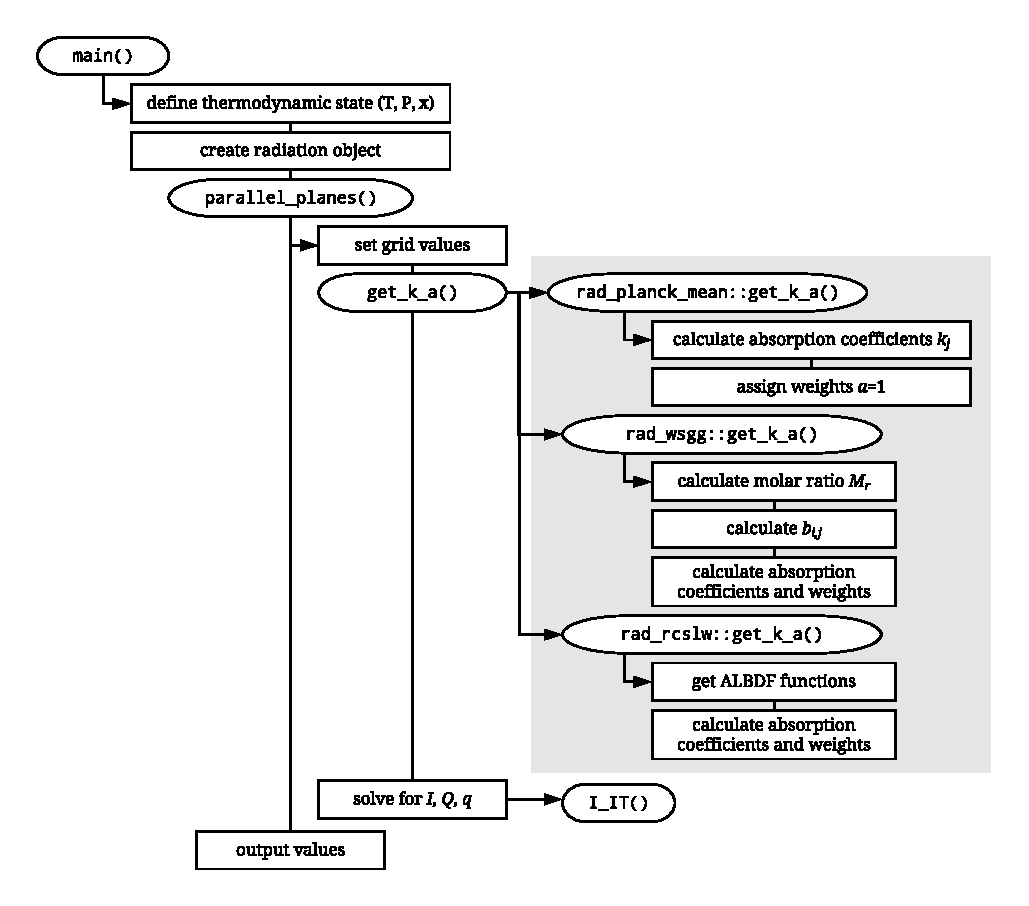
\includegraphics[width=\textwidth]{fig_radlib_structure.pdf}
	\end{center}
	\caption{Example workflow diagram. Highlighted areas are part of the RadLib library; other areas represent example infrastructure for using the package.}
\label{fig:flowchart}
\end{figure}
%

The RadLib source code is build around a base class called \texttt{rad} from which the individual property models, e.g., \texttt{rad\textunderscore rcslw}, inherit.
To extend RadLib to include new radiative property models, a user would create a new derived class for the model that inherits from the \texttt{rad} base class. The interface functions \texttt{get\textunderscore k\textunderscore a} and \texttt{get\textunderscore k\textunderscore a\textunderscore oneband} would be reimplemented in the new model. Additional functions and capabilities could be added as desired. The Fortran and Python interface codes consist of wrapper functions to the underlying C++. These can be easily extended by paralleling the existing interface functions. 

%%%%%%%%%%%%%%%%%%%%%%%%%%%%%%%%%%%%%%%%%%%%%%%%%%%%%%%%%%%%%%%%%%%%%%%%%%%%%%%%

\section{Examples} \label{s:Examples}

The RadLib package includes several example cases that illustrate the behavior of the models and interfaces. The examples compare the PM, WSGG, and RCSLW models via output heat flux $q$ or volumetric heat source $Q$ in one-dimensional configurations with varying gas compositions and temperatures. 
The RTE is solved between two parallel plates with a ray-tracing code, included in the RadLib package. Each case's results is presented alongside the line-by-line (LBL) data from its respective reference. 

Table~\ref{t:examples} summarizes the example cases. Each case is labeled according to its source---Solvojov et al. \cite{Solovjov_2017} (S), Bordbar et al. \cite{Bordbar_2020} (B), or Solovjov et~al. \cite{Solovjov_2001} (Sb)---and the number of each example corresponds to the example number in its respective reference. Each example case consists of one or more gas layers ("slabs") bounded by black walls. 
Example S1 consists of two adjacent gas layers with identical species compositions: one hot layer of constant thickness and one cold layer of varying thickness. 
In Example S2, the two gas layers are isothermal but differ in the value of the \ce{CO2} mole fraction, where the layer thickness of the ``thin'' slab (with the smaller \ce{CO2} mole fraction) varies.
Example S3 applies parabolic temperature and \ce{H2O} mole fraction profiles across a single gas layer. 
Example S4 divides the gas into three equally-spaced layers and applies a triangular temperature profile to the middle layer and a constant temperature to the two outer layers.
Example S5 uses a half-sinusoid temperature profile that decreases from 1500 to 500 K applied to a single gas layer of constant species composition.
Example B3 has symmetric temperature and H$_2$O mole fraction profiles with central peaks of 1800 K and 1, respectively (with $x_{CO2}=1-x_{H2O}$). 
Example Sb1 consists of a single gas with a uniform temperature and composition profile and soot radiation. 
%
\begin{table}
    \caption{Summary of example cases. All cases use $P=1$ atm and black walls.}
    \label{t:examples}
    \centering
    \resizebox{\textwidth}{!}{
    \begin{tabular}{c l l c c c c}
        \hline
        Example & T(K)                          & $x_{H2O}$  $x_{CO2}$ (mole frac.)               & L (m)   & $T_{walls}$ (K) & Ref.\\
        \hline
        S1 & $T(x<0.5)=2000$; $T(x>0.5)=300$    & $x_{CO2}=0.1$, $x_{H2O}=0.2$                    & 0.5-2.5 & cold, cold	& \cite{Solovjov_2017}     \\
        S2 & T=1000                             & $x_{CO2}(x<0.5)=0.4$, $x_{CO2}(x>0.5)=0.1$      & 0.5-2.5 & cold, cold & \cite{Solovjov_2017}    \\
           &                                    & $x_{H2O}=0.0$                                   &         &                \\
        S3 & $T(x) = 4000x(L-x)/L^2 + 800$      & $x_{H2O}(x) = 0.8x(L-x)/L^2 + 0.12$             & 1       & 800, 800 & \cite{Solovjov_2017}      \\
           &                                    & $x_{CO2}=0$                                     &         &                \\
        S4 & middle third triangular to 2500    & $x_{H2O}=0.1$, $x_{CO2}=0$                      & 0.3     & 500, 500 & \cite{Solovjov_2017}      \\
        S5 & $T(x) = 1000 + 500\cos(\pi x/L)$ 	 & $x_{H2O}=0.1$, $x_{CO2}=0$                      & 2       & 1500, 500 & \cite{Solovjov_2017}     \\
        B3 & $T(x) = 400 + 1400\sin(\pi x/L)^2$ & $x_{H2O}(x) = 0.0001 + 0.9999\sin(\pi x/L)^2$	& 1       & 400, 400 & \cite{Bordbar_2020}      \\
           &                                    & $x_{CO2}=1-x_{H2O}$                             	&         &                \\
        Sb1& $T = 1000$                         & $x_{H2O} = 0.2$, $x_{CO2}=0.1$, $x_{CO}=0.03$   	& 1       & cold, cold & \cite{Solovjov_2001}    \\
        \hline
    \end{tabular}
    }
\end{table}
%

The examples are provided with the RadLib code and implemented in both C++ and Python. A Juptyer notebook is provided with the Python examples that runs the examples, displays the plots, and saves the plots to PDF files. Python and Cython versions of the one-dimensional solver \texttt{parallel\textunderscore planes.py} are provided for convenience. 

These cases are intended to illustrate the use of the RadLib library and are not exhaustive. Details about these examples and their motivations can be found in their respective references. Comparison of these results to the LBL data, shown here, serve as model validation. For WSGG and RCSLW, direct comparison (not shown) of RadLib was made to examples presented in the model references with identical results (up to the resolution of the available data), which serves as verification of the implementation.

%%%%%%%%%%%%%%%%%%%%%%%%%%%%%%%%%%%%%%%%%%%%%%%%%%%%%%%%%%%%%%%%%%%%%%%%%%%%%%%%

\section{Results and Discussion} \label{s:discussion}

Figures~\ref{f:examples} and~\ref{f:exSb1} display comparative results for the PM, WSGG, and RCSLW models implemented by RadLib in the example case configurations summarized in Table~\ref{t:examples}. These plots are included to demonstrate the examples that are provided with the code, and to compare the models to give an indication of their relative accuracy. In all examples, the RCSLW model data is computed using four gray gases ($n=4$) and one clear gas for consistent comparison to the WSGG model, with the exception of Example S5, in which the number of gray gases in the RCSLW model is varied. The RCSLW model is initialized using the mean temperature and composition on the domain for all cases except Example S5, which uses the maximum temperature. 
%
\begin{figure}
    \begin{center}
    \begin{tabular}{c c}
        Example S1 & Example S2 \\
        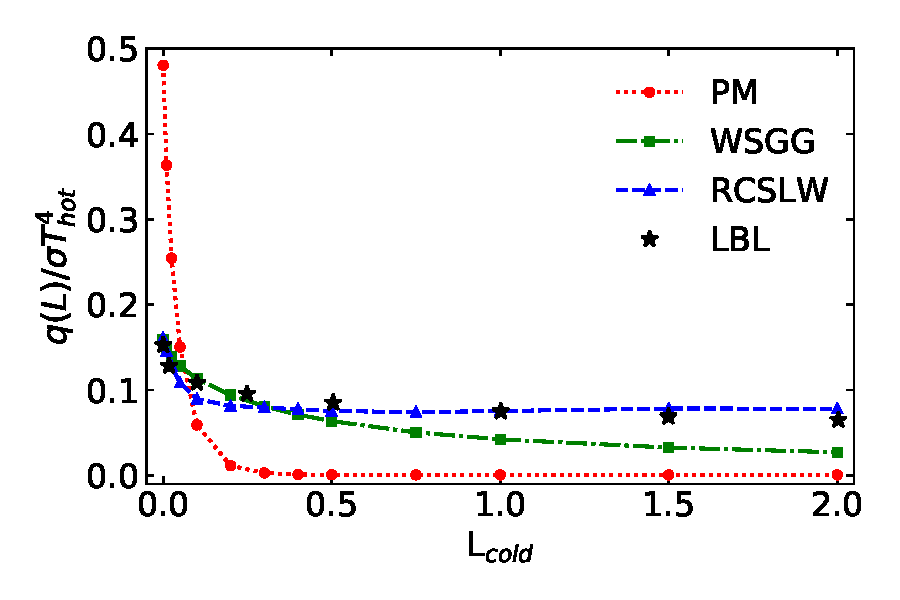
\includegraphics[width=2.75 in]{fig_ex_S1.pdf} &
        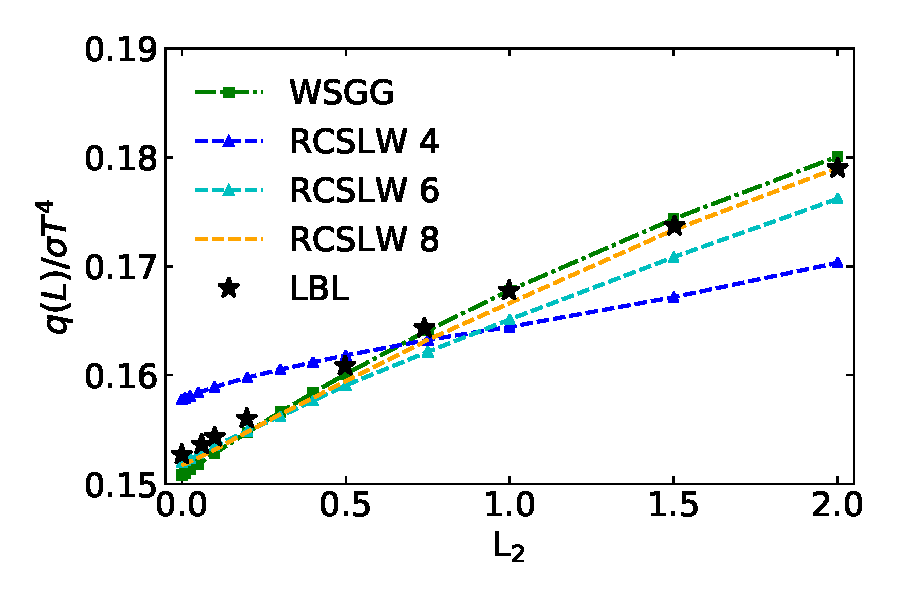
\includegraphics[width=2.75 in]{fig_ex_S2b.pdf} \\
        Example S3 & Example S4 \\
        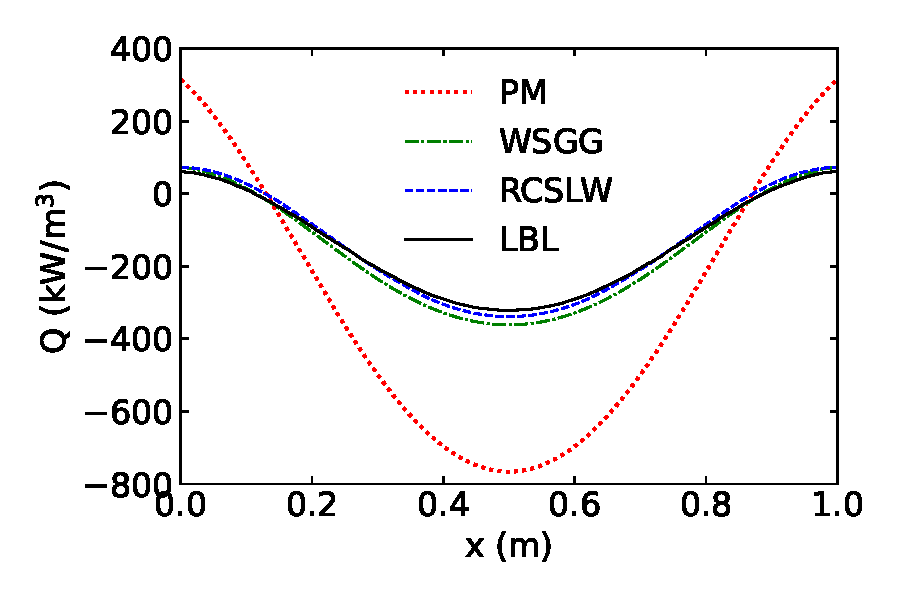
\includegraphics[width=2.75 in]{fig_ex_S3a.pdf} &
        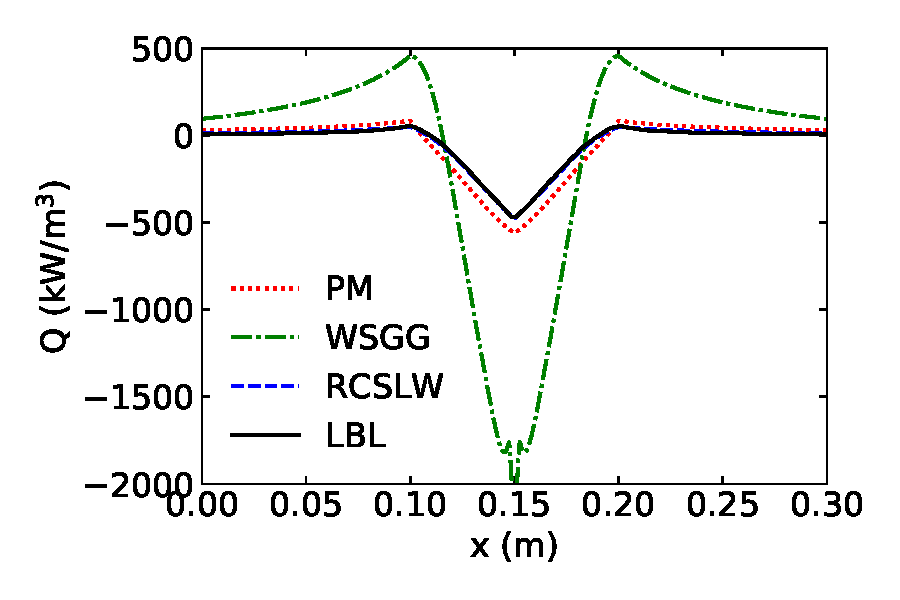
\includegraphics[width=2.75 in]{fig_ex_S4a.pdf} \\
        Example S5 & Example B3 \\
        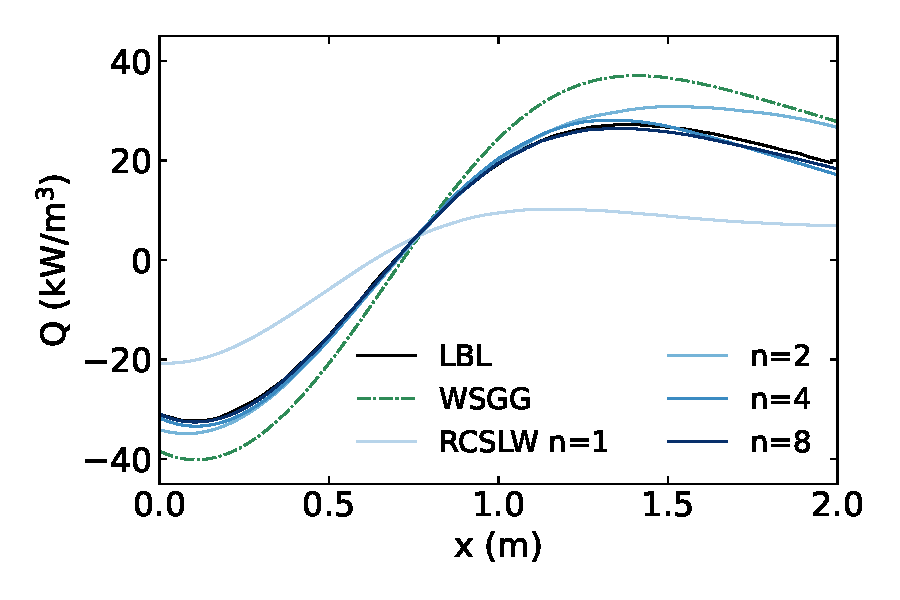
\includegraphics[width=2.75 in]{fig_ex_S5c.pdf} &
        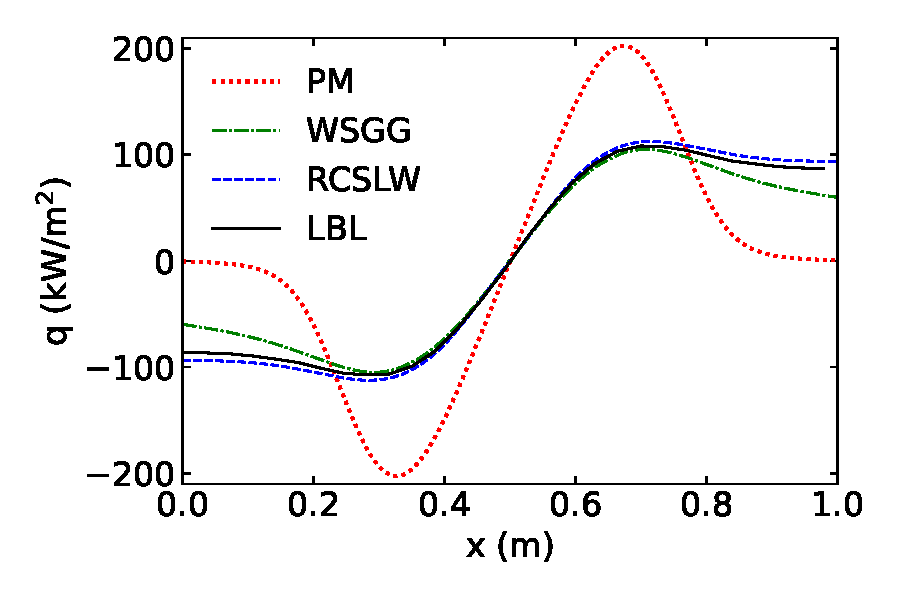
\includegraphics[width=2.75 in]{fig_ex_B3.pdf}
    \end{tabular}
    \caption{Results for Examples S1-S5 and B3 summarized in Table~\ref{t:examples}.}
    \label{f:examples}
    \end{center}
\end{figure}
%
\begin{figure}
    \begin{center}
        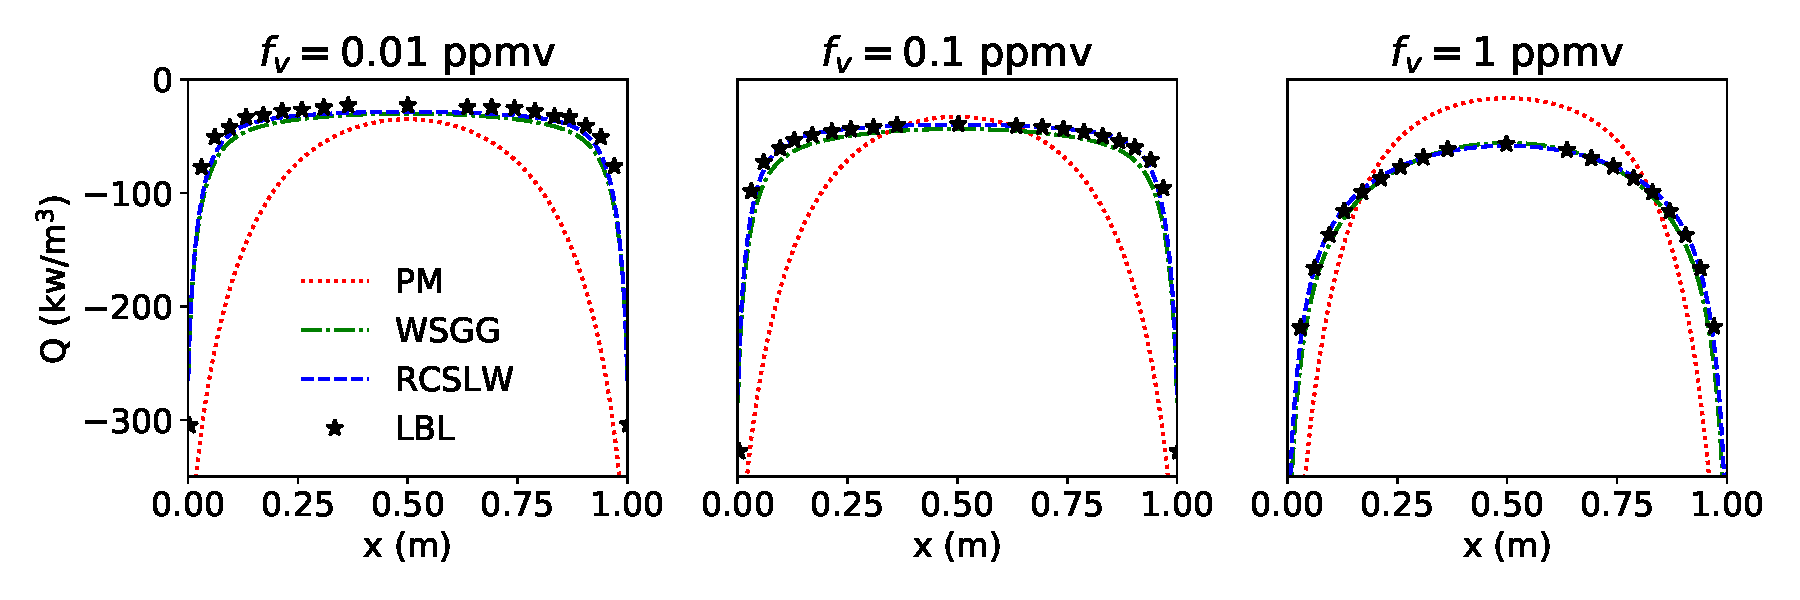
\includegraphics[width=5.5 in]{fig_ex_Sb1.pdf}
    \caption{Results for Example Sb1 summarized in Table~\ref{t:examples}.}
    \label{f:exSb1}
    \end{center}
\end{figure}
%

In general, the PM model performs poorly compared to the WSGG and RCSLW models and the LBL data. The results show that the PM model tends to exaggerate the trends displayed by the other models. The PM data mimics the shape of the other curves in Example S5 as well, but the curve is off-scale and omitted for clarity. For the PM model in Example S5, $Q$ varies from around -80 kW/m$^3$ at $x=0$ to a peak of 200 kW/m$^3$ at x=$1.5$ m and drops to 100 kW/m$^3$ at $x=2$ m. 
In Example S2, the PM value of $q(L)/\sigma T^4$ is off the scale at an essentially constant value of unity. The PM absorption coefficient is 27.4 atm$^{-1}$m$^{-1}$, which results in a calculated optical thicknesses of 0.09 and 0.36 m in the thick and thin layers, respectively. These values are small compared to the domain sizes greater than 0.5 m that are considered in Example S2.
%, which coincides with the PM model's use of the optically thin approximation, but the high error in its predictions of radiative heat flux relative to the LBL data indicates that neither the optically thin approximation nor absorption coefficients calculated with this model are accurate for this case. 
Example S3 is the clearest illustration of the PM model's deficiencies as discussed in Section~\ref{s:planckmean}: the PM model overpredicts radiative heat loss at the high temperatures that characterize most combustion processes. 

The WSGG model closely follows the trends of the LBL data for all examples, and in most examples gives reasonable quantitative agreement. This is especially true for Example S2, S4, and B3. For example S5, the WSGG model shows peak errors of around 50\%, and somewhat higher in Example S1. The heat flux near the boundaries in Example B3 is low by around 30\%. The RCSLW model gives results in very close agreement to the LBL data for all examples. A notable exception is example S2, where the heat flux at the right boundary is not well-predicted for four gray gases. The heat flux does converge to the LBL results when the number of gray gases increases. This behavior was not discussed in \cite{Solovjov_2017} where 24 gray gases were used. The WSGG model is very close to the LBL data for this case. The good agreement is likely a result of the simplicity of this case that is isothermal with pure \ce{CO2} at uniform concentration in either of the two adjacent gas slabs.
The RCSLW model is sensitive to the number of gray gases used, as illustrated in Figure~\ref{f:examples} by Examples S2 and S5. The difference in accuracy between $n=2$ and $n=8$ gray gases is small for all of the example cases and typically falls within the margin of error represented by the WSGG model's deviation from the LBL data. 
The RCSLW model also depends on the value of the chosen reference temperature that is used to set the ALBDF grid. In Example S5, the RCSLW model does not converge to the LBL data at $x>0.5$ m when the domain average temperature was used.

%The WSGG model gives somewhat accurate but inconsistent results for the example cases considered here. In Examples S1, S3, S5, B3, and Sb1, it behaves as expected, producing results that are closer to the LBL data than those produced by the PM model but fall short of the RCSLW model's level of accuracy. In general, the WSGG model appears to perform best at intermediate temperatures and deviates from the desired behavior at boundary conditions, but this is not universal. For example, the WSGG model shows uncharacteristically high accuracy in Example S2; its results with four gray gases are comparable in accuracy to the RCSLW model's performance using eight or more gray gases. In contrast, the WSGG model performs exceptionally poorly in Example S4, in which it deviates from the LBL data by nearly an order of magnitude at its largest. 
%The WSGG model, alongside with the PM model, is primarily empirical and contains little to no representative physics, which could explain the unexpected behavior in Examples S2 and S4. Given that all of the example cases use parameters within those specified for the WSGG model in the literature \cite{Bordbar_2014,Bordbar_2020}, neither anomalous result has an obvious source. While we cannot offer an explanation for the WSGG model's inconsistent performance, it serves to underscore the importance of individual model validation on a case-by-case basis, a task potentially made easier with tools like RadLib. 

%The RCSLW model displays the most accurate results of the three implemented property models when compared to LBL data, capturing the relevant trends without exaggerating them. It is, however, the most difficult of the three models to implement and requires either correlated or tabulated spectral data to draw from. 
%The RCSLW model can be sensitive to the number of gray gases used, illustrated in Figure~\ref{f:examples} by Examples S2 and S5. The difference in accuracy between $n=2$ and $n=8$ gray gases is small for all of the example cases and typically falls within the margin of error represented by the WSGG model's deviation from the LBL data. Example S2 shows the most prominent variations in predicted radiative heat flux based on changes in the number of gray gases, improving drastically in agreement to the LBL data with the addition of just four gray gases. RCSLW model convergence can also vary with the value of the chosen reference temperature; in Example S5, for instance, the RCSLW model converges to the LBL data if it is initialized with the maximum rather than the average temperature on the domain. When treated properly, however, the RCSLW model provides the most accurate results of all of the radiation property models considered here. 

Figure~\ref{f:exSb1} shows the results from Example Sb1, which considers three magnitudes of the soot volume fraction in addition to the radiating gas. Both the WSGG and RCSLW models perform accurately in all three cases, but the PM model displays significant deviations from the LBL data. In sooting flames, soot acts as a significant source and sink of radiation, and its radiative properties differ significantly from those of the participating gaseous species. Soot reactions and transport are both sensitive to and strongly influence local variations in flame temperature and gas composition, forming a feedback loop in which accurate prediction of both gas and soot radiative properties becomes critical to predicting flame properties and behavior, particularly late-stage flame phenomena such as flame sheet breakthrough, smoke production, and extinction and reignition processes.
%The agreement produced by RadLib's approach to soot radiation in Example Sb1 is an encouraging step toward accurate, detailed treatment of soot's radiative properties in complex combustion simulations. 



%%%%%%%%%%%%%%%%%%%%%%%%%%%%%%%%%%%%%%%%%%%%%%%%%%%%%%%%%%%%%%%%%%%%%%%%%%%%%%%%

\subsection{CFD Results} \label{s:cfd}

The RadLib model was coupled to the Fire Dynamics Simulator (FDS) code developed at NIST \cite{FDS}. FDS is written in Fortran, and the Fortran interface of Radlib was used for simulations. FDS includes several radiative models, but the spectral WSGG model coupled to a finite volume discrete ordinates model is used here. This was done by editing the \texttt{radi.f90} file. A \texttt{use rad\textunderscore module} statement is included and the functions \texttt{A\textunderscore WSGG} and \texttt{KAPPA\textunderscore WSGG} were replaced with calls to RadLib's \texttt{get\textunderscore k\textunderscore a\textunderscore oneband}. The \texttt{oneband} version was used because FDS does an outer iteration over the bands/gases, computing properties at a given band for each grid point. 

FDS includes a number of validation cases. Here, we compare to the FM Burner case. The configuration is a vertically fired gas burner with various fuels and with a coflow oxidizer stream of varying nitrogen dilution. The burner has outer and inner diameters of 15.2 and 13.7 cm and is near the floor in the center of a 1.22 by 1.22 by 1.83 m tall compartment. The heat release rate was 10 kW and included a 1 kW pilot in a surrounding ring. The coflow oxidizer was fed through the floor. Simulations performed here used the ethylene fuel with 20.9\% \ce{N2} oxidizer (i.e., air). Further FDS model and case simulation details are provided in the FDS validation and user guides \cite{FDS}.

Figure~\ref{f:fds} shows results of the simulation with comparison to experimental data. Three radiation models were included: the FDS default model, and the RCSLW and WSGG models from RadLib (both using four gray gases and one clear gas). 
The FDS default model uses a single gray gas with a composition and temperature dependent absorption coefficient computed from RADCAL. Further details are provided in the FDS user guide \cite{FDS}. 
Figure~\ref{f:fds}a shows radial profiles of mean temperature at two vertical positions. The models produce centerline temperature differences of about 80 K (7\%) between the RCSLW and the WSGG at z=2.5D, and 90 K (12\%) at z=3.5D. The differences are lower at lower points in the flame since the effect of radiation on temperature is cumulative. Figure~\ref{f:fds}b plots height versus radiative emission per unit length along the centerline with the spread in radiative emission around the peak values being 1.3 kW/m (11\%).
%
\begin{figure}
    \begin{center}
    \begin{tabular}{c c}
        (a) & (b) \\
        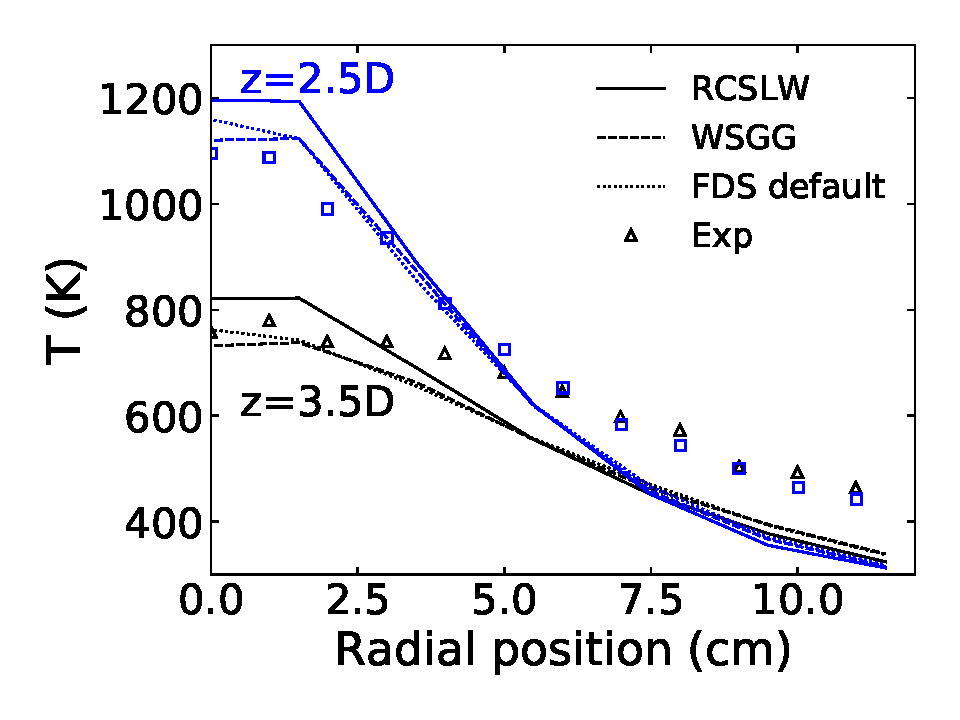
\includegraphics[width=2.5 in]{fig_fds_T_mean.pdf} &
        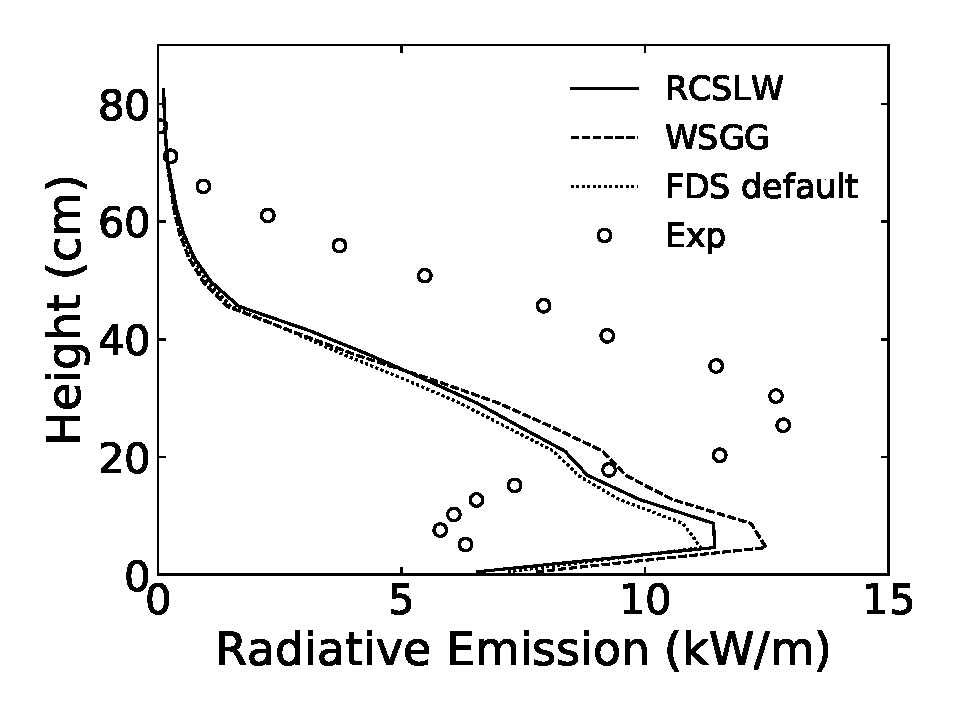
\includegraphics[width=2.5 in]{fig_fds_rad_mean.pdf}
    \end{tabular}
    \caption{Radial profiles of mean temperature at two heights (a), and height versus radiative emission (b) for FDS simulations of the FM Burner validation case comparing three models to experimental data.}
    \label{f:fds}
    \end{center}
\end{figure}
%

%%%%%%%%%%%%%%%%%%%%%%%%%%%%%%%%%%%%%%%%%%%%%%%%%%%%%%%%%%%%%%%%%%%%%%%%%%%%%%%%

\subsection{Computational Cost} \label{s:cost}

In addition to comparing model attributes and performance, we evaluated and compared the computational cost of the implemented radiation property models. 
Calculations were performed on a 4 GHz Quad Core Intel Core i7 iMac, version 10.15.7; the results, normalized by the cost of the WSGG model, are summarized in Figure~\ref{f:cost}. 
In the results presented, only the cost of evaluating the solution was included; model initialization and input/output costs were neglected. In the results including the ray-tracing solver, the same number of rays and grid points is used in all calculations.

Figure~\ref{f:cost}a displays the relative cost to compute the gas properties $k$ and $a$, represented by the time required to execute the C++ function \texttt{get\textunderscore k\textunderscore a()}, averaged over one million evaluations. The results for each model are normalized by the WSGG model, which required an average of 8.0E-7~s. Relative to the WSGG model, the cost to evaluate the gas properties with the PM model was 0.098. The RCSLW model was evaluated with $n=1$, 2, 4, and 8 gray gases, which resulted in relative costs of 1.9, 4.9, 9.4, and 18, respectively. The cost of the RCSLW model is very nearly proportional to the number of gray gases considered.
%
\begin{figure}
    \begin{center}
    \begin{tabular}{c c}
        (a) & (b) \\
        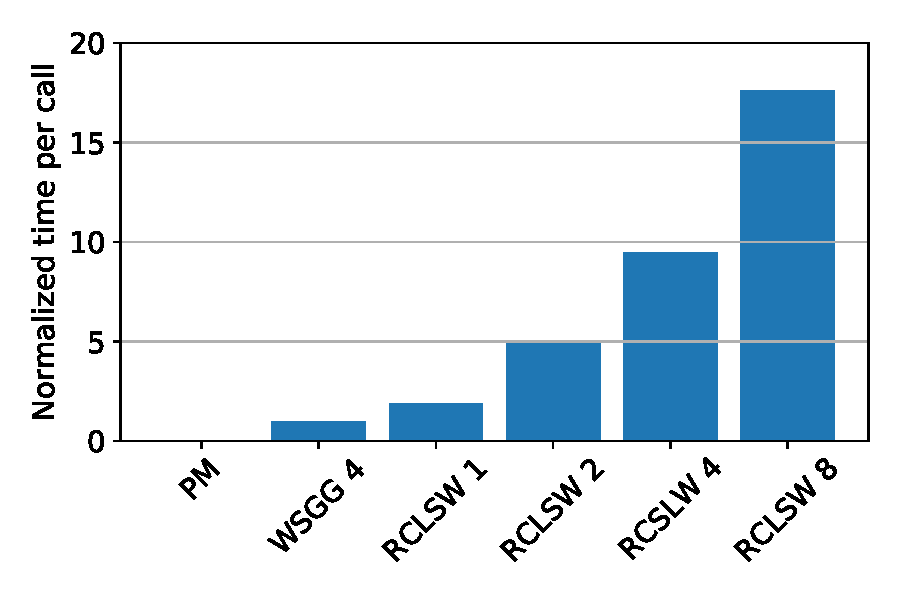
\includegraphics[width=2.5 in]{fig_getka_c++.pdf} &
        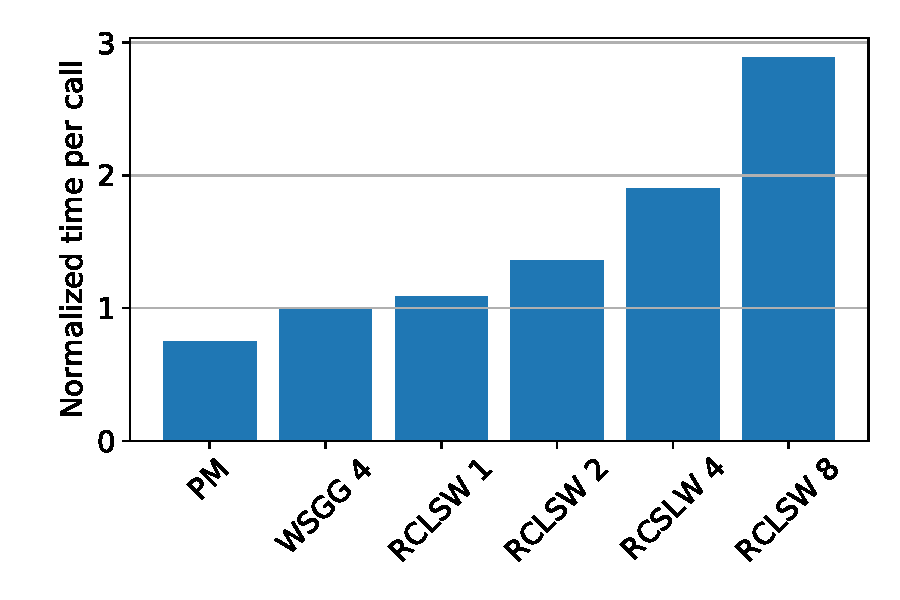
\includegraphics[width=2.5 in]{fig_exS3_c++.pdf}
    \end{tabular}
    \caption{Relative computational cost to (a) evaluate gas properties only and (b) run Example S3, including the ray-tracing solver. Results are normalized by the cost of the WSSG model for each case.}
    \label{f:cost}
    \end{center}
\end{figure}
%

Figure~\ref{f:cost}b shows the cost to evaluate Example S3, which involves both evaluation of the gas properties and solution of the RTE using the provided ray-tracing solver. This is relavant because radiative property calculations are rarely done in isolation, but are part of a larger RTE solution, so that overall cost differences may be smaller than those of the property evalations themselves. This is consistent with the results of the figure and as follows. Relative to the WSGG model, which required 0.0079 s, the model costs for the PM model and the RCSLW model with $n=1$, 2, 4, 8 gray gases was approximately 0.75, 1.1, 1.4, 1.9, and 2.9, respectively. 
%In running Example S3, the overall solution cost using different property models is shown to vary much less than when evaluating gas properties alone due to the additional overhead of the ray-tracing solver in performing the calculations. 

Cost comparisons were also attempted with Python, but meaningful results are difficult to obtain when mixing Python and C++. In particular, the cost of a single evaluation of the gas properties is small and evaluating the gas properties in a Python loop results in the loop itself appearing to dominate the computational cost. Comparison between Python and C++ for Example S3 is somewhat more meaningful, but even here, for the six cases considered in Figure~\ref{f:cost} the cost only varied by about 4\%, indicating that the computational cost is dominated by Python wrapper itself rather than by the underlying C++ model evaluations or solver. The cost of the WSGG model was 0.6~s, which is 7.6 times slower than the C++ version. It is possible that optimizing the Cython interface could improve the speed and relative cost of using Python with RadLib, but RadLib's Python interface and examples are mainly intended to demonstrate the library's use and provide a convenient interface, rather than serve as a point of incorporation into detailed CFD calculations.%, which rarely employ Python.

%%%%%%%%%%%%%%%%%%%%%%%%%%%%%%%%%%%%%%%%%%%%%%%%%%%%%%%%%%%%%%%%%%%%%%%%%%%%%%%%

\section{Conclusions} \label{s:conclusions}

Radiative heat transfer phenomena are historically difficult to model and implement in CFD calculations due to their high level of conceptual and mathematical complexity and potentially large computational cost. Many combustion CFD studies either neglect radiative heat transfer modeling or employ oversimplified models that do not accurately represent combustion systems. Most combustion processes of interest to engineers and researchers, however, involve significant radiative heat transfer, and simulations require robust radiative modeling, which includes both radiation property modeling and solution approaches for the radiative transfer equation, to yield accurate results. 

RadLib is a C++ library of radiation property models developed to facilitate implementing radiative property models in CFD simulations. At present, it includes three major radiation property models---Planck Mean (PM) absorption coefficients using the optically thin approximation, the weighted sum of gray gases (WSGG) model, and the rank-correlation spectral line weighted-sum-of-gray-gases (RCSLW) model---but its design and C++, Python, and Fortran interfaces permit expansion to additional property models. Each of the implemented models has been validated and the library's structure and functionality has been outlined. 

In addition to the library itself, the RadLib package includes several illustrative example cases in a one-dimensional parallel planes geometry using a simple ray tracing solver to demonstrate use of the library and validate model implementation. Results are compared to line-by-line (LBL) solutions. In general, the RCSLW model outperforms both the PM and WSGG models in terms of accuracy at the expense of computational cost. Under appropriate conditions, the WSGG model can also produce accurate results at significantly lower computational cost, but may perform inconsistently under certain conditions. In general, the PM model is adequate in situations to which the optically thin approximation can be reasonably applied, but does not produce accurate results in any of the example cases presented here. 

RadLib is intended as a convenient access point for researchers who require radiation property modeling tools for combustion CFD, but could potentially be applied to research problems involving radiative heat transfer in other fields as well. RadLib is designed to facilitate and simplify the process of implementing and/or using radiative property models; it consolidates various model types into a single extensible library with a consistent framework, reducing some of the overhead associated with choosing, implementing, and testing radiation property models. Its framework can be used to implement and validate new models as well as compare existing models under consistent conditions. By facilitating model comparison through a common interface, RadLib can provide a practical means of testing specific modeling approaches without the restrictions imposed by large-scale CFD simulations. With RadLib, we believe that researchers will be able to put more of their time and effort into meaningful results rather than code or model development for radiative heat transfer in combustion CFD. 

%%%%%%%%%%%%%%%%%%%%%%%%%%%%%%%%%%%%%%%%%%%%%%%%%%%%%%%%%%%%%%%%%%%%%%%%%%%%%%%%

\section{Declaration of Competing Interests} \label{s:coi}

The authors declare that they have no known competing financial interests or personal relationships that could have appeared to influence the work reported in this paper.


%%%%%%%%%%%%%%%%%%%%%%%%%%%%%%%%%%%%%%%%%%%%%%%%%%%%%%%%%%%%%%%%%%%%%%%%%%%%%%%%

\section*{Acknowledgements} \label{sec:acknowledgements}

The authors extend special thanks to Hadi Bordbar for assistance with the WSGG model and to Vladimir Solovjov and Brent Webb for their insights and assistance with the RCSLW model. 
This research did not receive any specific grant from funding agencies in the public, commercial, or
not-for-profit sectors.

%%%%%%%%%%%%%%%%%%%%%%%%%%%%%%%%%%%%%%%%%%%%%%%%%%%%%%%%%%%%%%%%%%%%%%%%%%%%%%%%

\bibliographystyle{elsarticle-num} 
\bibliography{references} 

%\begin{thebibliography}{10}
%\expandafter\ifx\csname url\endcsname\relax
%  \def\url#1{\texttt{#1}}\fi
%\expandafter\ifx\csname urlprefix\endcsname\relax\def\urlprefix{URL }\fi
%\expandafter\ifx\csname href\endcsname\relax
%  \def\href#1#2{#2} \def\path#1{#1}\fi
%
%\bibitem{Hottel_1967}
%H.~Hottel, A.~Sarofim, Radiative Transfer, {McGraw-Hill}, New York, 1967.
%
%\bibitem{Modest_2013}
%M.~F. Modest, Radiative Heat Transfer, third edition, {Academic Press},
%  New York, 2013.
%  
%\bibitem{Modest_2016}
%M.~F. Modest, D.~C. Haworth, Radiative Heat Transfer in Turbulent Combustion Systems, {Springer}, New York, 2016.
%
%\bibitem{Smith_2003}
%N.~Smith, J.~Gore, J.~Kim, Q.~Tang,
%  \href{https://tnfworkshop.org/radiation/}{{TNF} workshop radiation models}
%  (2003).
%\newline\urlprefix\url{https://tnfworkshop.org/radiation/}
%
%\bibitem{Grosshandler_1993}
%W.~L. Grosshandler, {RADCAL}: A narrow-band model for radiation calculations in
%  a combustion environment: Nist technical note 1402.
%
%\bibitem{Barlow_2001}
%R.~S. Barlow, A.~N. Karpetis, J.~H. Frank, J.-Y. Chen, Scalar profiles and {NO}
%  formation in laminar opposed-flow partially premixed methane/air flames,
%  Combustion and Flame 127~(3) (2001) 2102--2118.
%\newblock \href {http://dx.doi.org/10.1016/S0010-2180(01)00313-3}
%  {\path{doi:10.1016/S0010-2180(01)00313-3}}.
%
%\bibitem{Barlow_1999}
%R.~Barlow, N.~Smith, J.~Chen, R.~Bilger,
%  \href{http://www.sciencedirect.com/science/article/pii/S0010218098000716}{Nitric
%  oxide formation in dilute hydrogen jet flames: isolation of the effects of
%  radiation and turbulence-chemistry submodels}, Combustion and Flame 117~(1-2)
%  (1999) 4--31.
%\newblock \href {http://dx.doi.org/10.1016/S0010-2180(98)00071-6}
%  {\path{doi:10.1016/S0010-2180(98)00071-6}}.
%\newline\urlprefix\url{http://www.sciencedirect.com/science/article/pii/S0010218098000716}
%
%\bibitem{Frank_2000}
%J.~H. Frank, R.~S. Barlow, C.~Lundquist, Radiation and nitric oxide formation
%  in turbulent non-premixed jet flames, Proceedings of the Combustion Institute
%  28~(1) (2000) 447--454.
%\newblock \href {http://dx.doi.org/10.1016/S0082-0784(00)80242-8}
%  {\path{doi:10.1016/S0082-0784(00)80242-8}}.
%
%\bibitem{Zhu_2002}
%X.~Zhu, J.~Gore, A.~N. Karpetis, R.~S. Barlow,
%  \href{http://www.sciencedirect.com/science/article/pii/S0010218002003413}{The
%  effects of self-absorption of radiation on an opposed flow partially premixed
%  flame}, Combustion and Flame 129~(3) (2002) 342--345.
%\newblock \href {http://dx.doi.org/10.1016/S0010-2180(02)00341-3}
%  {\path{doi:10.1016/S0010-2180(02)00341-3}}.
%\newline\urlprefix\url{http://www.sciencedirect.com/science/article/pii/S0010218002003413}
%
%\bibitem{Coelho_2002}
%P.~J. Coelho, O.~J. Teerling, D.~Roekaerts, Spectral radiative effects and
%  turbulence-radiation-interaction in sandia flame {D}, in: {Barlow, Robert S.,
%  Pope, Stephan B., Masri, Assaad R., Oefelein, Joseph C.} (Ed.), The
%  Proceedings of the Sixth International Workshop on Measurement and
%  Computation of Turbulent Nonpremixed Flames, 2002.
%
%\bibitem{Bordbar_2014}
%M.~H. Bordbar, G.~Wecel, T.~Hyppanen, A line by line based weighted sum of gray
%  gases model for inhomogeneous {CO$_2$–H$_2$O} mixture in oxy-fired
%  combustion, Combustion and Flame 161~(9) (2014) 2435--2445.
%\newblock \href {http://dx.doi.org/10.1016/j.combustflame.2014.03.013}
%  {\path{doi:10.1016/j.combustflame.2014.03.013}}.
%
%\bibitem{Bordbar_2020}
%H.~Bordbar, G.~C. Fraga, S.~Hostikka,
%  \href{http://www.sciencedirect.com/science/article/pii/S0735193319302660}{An
%  extended weighted-sum-of-gray-gases model to account for all {CO$_2$-H$_2$O}
%  molar fraction ratios in thermal radiation}, International Communications in
%  Heat and Mass Transfer 110 (2020) 104400.
%\newblock \href {http://dx.doi.org/10.1016/j.icheatmasstransfer.2019.104400}
%  {\path{doi:10.1016/j.icheatmasstransfer.2019.104400}}.
%\newline\urlprefix\url{http://www.sciencedirect.com/science/article/pii/S0735193319302660}
%
%\bibitem{Rothman_2010}
%L.~S. Rothman, I.~E. Gordon, R.~J. Barber, H.~Dothe, R.~R. Gamache, A.~Goldman,
%  V.~I. Perevalov, S.~A. Tashkun, J.~Tennyson,
%  \href{http://www.sciencedirect.com/science/article/pii/S002240731000169X}{{HITEMP},
%  the high-temperature molecular spectroscopic database}, Journal of
%  Quantitative Spectroscopy {\&} Radiative Transfer 111~(15) (2010) 2139--2150.
%\newblock \href {http://dx.doi.org/10.1016/j.jqsrt.2010.05.001}
%  {\path{doi:10.1016/j.jqsrt.2010.05.001}}.
%\newline\urlprefix\url{http://www.sciencedirect.com/science/article/pii/S002240731000169X}
%
%\bibitem{Solovjov_2016}
%V.~P. Solovjov, F.~Andr{\'e}, D.~Lemonnier, B.~W. Webb, The generalized {SLW}
%  model, Journal of Physics: Conference Series 676 (2016) 1--36.
%
%\bibitem{Solovjov_2017}
%V.~P. Solovjov, F.~Andr{\'e}, D.~Lemonnier, B.~W. Webb, The rank correlated
%  {SLW} model of gas radiation in non-uniform media, Journal of Quantitative
%  Spectroscopy {\&} Radiative Transfer 197 (2017) 26--44.
%\newblock \href {http://dx.doi.org/10.1016/j.jqsrt.2017.01.034}
%  {\path{doi:10.1016/j.jqsrt.2017.01.034}}.
%
%\bibitem{Badger_2019}
%J.~Badger, B.~W. Webb, V.~P. Solovjov, An exploration of advanced {SLW}
%  modeling approaches in comprehensive combustion predictions, Combustion
%  Science and Technology 012022~(676) (2019) 1--17.
%\newblock \href {http://dx.doi.org/10.1080/00102202.2019.1678907}
%  {\path{doi:10.1080/00102202.2019.1678907}}.
%
%\bibitem{Solovjov_2000}
%V.~P. Solovjov, B.~W. Webb, {SLW} modeling of radiative transfer in
%  multicomponent gas mixtures, Journal of Quantitative Spectroscopy and
%  Radiative Transfer 65 (2000) 655--672.
%
%\bibitem{Solovjov_2001}
%V.~P. Solovjov, B.~W. Webb, An efficient method for modeling radiative transfer
%  in multicomponent gas mixtures with soot, Transactions of the ASME 123 (2001)
%  450--457.
%
%\bibitem{Solovjov_2008}
%V.~P. Solovjov, B.~W. Webb, Multilayer modeling of radiative transfer by {SLW}
%  and {CW} methods in non-isothermal gaseous medium, Journal of Quantitative
%  Spectroscopy and Radiative Transfer 109~(2) (2008) 245--257.
%\newblock \href {http://dx.doi.org/10.1016/j.jqsrt.2007.08.015}
%  {\path{doi:10.1016/j.jqsrt.2007.08.015}}.
%
%\bibitem{Solovjov_2011}
%V.~P. Solovjov, D.~Lemonnier, B.~W. Webb, The {SLW}-1 model for efficient
%  prediction of radiative transfer in high temperature gases, Journal of
%  Quantitative Spectroscopy and Radiative Transfer 112~(7) (2011) 1205--1212.
%\newblock \href {http://dx.doi.org/10.1016/j.jqsrt.2010.08.009}
%  {\path{doi:10.1016/j.jqsrt.2010.08.009}}.
%
%\bibitem{Solovjov_2014}
%V.~P. Solovjov, D.~Lemonnier, B.~W. Webb, Extension of the exact {SLW} model to
%  non-isothermal gaseous media, Journal of Quantitative Spectroscopy and
%  Radiative Transfer 143 (2014) 83--91.
%\newblock \href {http://dx.doi.org/10.1016/j.jqsrt.2013.10.008}
%  {\path{doi:10.1016/j.jqsrt.2013.10.008}}.
%
%\bibitem{Webb_2018}
%B.~W. Webb, V.~P. Solovjov, F.~Andr{\'e}, An exploration of the influence of
%  spectral model parameters on the accuracy of the rank correlated slw model,
%  Journal of Quantitative Spectroscopy and Radiative Transfer 218 (2018)
%  161--170.
%\newblock \href {http://dx.doi.org/10.1016/j.jqsrt.2018.06.023}
%  {\path{doi:10.1016/j.jqsrt.2018.06.023}}.
%
%\bibitem{Pearson_2014}
%J.~Pearson, B.~Webb, S.~V.P., J.~Ma, Efficient representation of the absorption
%  line blackbody distribution function for {H$_2$O}, {CO$_2$}, and {CO} at
%  variable temperature, mole fraction, and total pressure, Journal of
%  Quantitative Spectrosopy and Radiative Transfer 138 (2014) 82--96.
%
%\bibitem{Brewster_1992}
%M.~Q. Brewster, Thermal Radiative Transfer and Properties, Wiley, 1992.
%
%\bibitem{Lee_1981}
%S.~C. Lee, C.~L. Tien, Optical constants of soot in hydrocarbon flames,
%  Symposium (International) on Combustion 18~(1) (1981) 1159--1166.
%\newblock \href {http://dx.doi.org/10.1016/S0082-0784(81)80120-8}
%  {\path{doi:10.1016/S0082-0784(81)80120-8}}.
%
%\bibitem{Stull_1960}
%V.~R. Stull, G.~N. Plass, Emissivity of dispersed carbon particles, Journal of
%  the Optical Society of America 50~(2) (1960) 121.
%\newblock \href {http://dx.doi.org/10.1364/JOSA.50.000121}
%  {\path{doi:10.1364/JOSA.50.000121}}.
%
%\bibitem{Dalzell_1969}
%W.~H. Dalzell, A.~F. Sarofim, Optical constants of soot and their application
%  to heat-flux calculations, Journal of Heat Transfer 91~(1) (1969) 100--104.
%\newblock \href {http://dx.doi.org/10.1115/1.3580063}
%  {\path{doi:10.1115/1.3580063}}.
%
%\bibitem{Howarth_1966}
%C.~R. Howarth, P.~J. Foster, M.~W. Thring (Eds.), The Effect of Temperature on
%  the Extinction of Radiation By Soot Particles, Begellhouse, 1966.
%\newblock \href {http://dx.doi.org/10.1615/IHTC3.1210}
%  {\path{doi:10.1615/IHTC3.1210}}.
%
%\bibitem{Chang_1990}
%H.-c. Chang, T.~T. Charalampopoulos, Determination of the wavelength dependence
%  of refractive indices of flame soot, Proceedings of the Royal Society of
%  London. Series A: Mathematical and Physical Sciences 430~(1880) (1990)
%  577--591.
%\newblock \href {http://dx.doi.org/10.1098/rspa.1990.0107}
%  {\path{doi:10.1098/rspa.1990.0107}}.
%
%\bibitem{Felske_1984}
%J.~D. Felske, T.~T. Charalampopoulos, H.~S. Hura, Determination of the
%  refractive indices of soot particles from the reflectivities of compressed
%  soot pellets, Combustion Science and Technology 37~(5-6) (1984) 263--283.
%\newblock \href {http://dx.doi.org/10.1080/00102208408923757}
%  {\path{doi:10.1080/00102208408923757}}.
%
%\bibitem{Williams_2007}
%T.~C. Williams, C.~R. Shaddix, K.~A. Jensen, J.~M. Suo-Anttila, Measurement of
%  the dimensionless extinction coefficient of soot within laminar diffusion
%  flames, International Journal of Heat and Mass Transfer 50~(7-8) (2007)
%  1616--1630.
%\newblock \href {http://dx.doi.org/10.1016/j.ijheatmasstransfer.2006.08.024}
%  {\path{doi:10.1016/j.ijheatmasstransfer.2006.08.024}}.
%
%\bibitem{Felske_1977}
%J.~Felske, T.~C.L., The use of the {M}ilne-{E}ddington absorption coefficient
%  for radiative heat transfer in combustion systems, ASME Journal of Heat
%  Transfer 99~(3) (1977) 633--647.
%
%\bibitem{Bordbar_personal}
%H.~Bordbar, personal communication.
%
%\bibitem{Chang_1984}
%S.~Chang, K.~Rhee, Blackbody radiation functions, International communictions
%  in Heat and Mass Transfer 11 (1984) 451--455.
%
%\bibitem{Stephens_2020}
%V.~Stephens, D.~Lignell, One-dimensional turbulence ({ODT}): computationally
%  efficient modeling and simulation of turbulent flows, Software{X} 13 (2020)
%  100641.
%\newblock \href {http://dx.doi.org/10.1016/j.softx.2020.100641}
%  {\path{doi:10.1016/j.softx.2020.100641}}.
%  
%\bibitem{Zhang_2002b}
%H.~Zhang, M.~F.~Modest, Evaluation of the Planck-mean absorption coefficients from HITRAN and HITEMP databases, Journal of Quantitative Spectroscopy \& Radiative Transfer 73~(6) (2002) 649--653.

%\end{thebibliography}

%%%%%%%%%%%%%%%%%%%%%%%%%%%%%%%%%%%%%%%%%%%%%%%%%%%%%%%%%%%%%%%%%%%%%%%%%%%%%%%%

\end{document}
\endinput

